%ACM DOCUMENT
\documentclass[acmtoms]{acmtrans2m}

\usepackage[utf8]{inputenc}
%PACKAGES FOR MATH SYMBOLS
\usepackage{amsmath}
\usepackage{amsfonts}
\usepackage{amssymb}

%PACKAGE FOR PICTURES
\usepackage{graphicx}

%PACKAGES FOR ALGORITHMS
\usepackage{algorithmicx}
\usepackage[ruled]{algorithm}
\usepackage{algpseudocode}
\usepackage{algc}
\newcommand{\New}{\textbf{new}}

\acmVolume{1}
\acmNumber{1}
\acmYear{12}
\acmMonth{July}

% New commands
\newcommand{\DP}[2]{\displaystyle\frac{\partial #1}{\partial #2}}
\newcommand{\ds}{\displaystyle}
\newcommand{\bi}[1]{\boldsymbol{\mathit{#1}}}
\newcommand{\bs}[1]{\boldsymbol{#1}}
\newcommand{\bv}[1]{\mathbf{#1}}
\renewcommand{\b}[1]{\boldsymbol{\mathit{#1}}}

%HEADER
\markboth{M. Costa et al.}{Design and Implementation of the Three-Dimensional Autonomous Leaves Graph}

%TITLE
\title{ Design and Implementation of the Three-Dimensional Autonomous Leaves Graph Data Structure}

%AUTHORS
% \author
% {
%     MAYCON DA COSTA$^{\textrm{\,a}}$, DENISE BURGARELLI$^{\textrm{\,b}}$,
%     RODNEY JOSU\'E BIEZUNER$^{\textrm{\,b}}$ RAFAEL SACHETTO OLIVEIRA \and WAGNER MEIRA
%     JR.$^{\textrm{\,a}}$, Universidade Federal de Minas Gerais\\
%     RODRIGO WEBER DOS SANTOS, Universidade Federal de Juiz de Fora
%
% }
 \author
 {
     MAYCON DA COSTA, DENISE BURGARELLI,
     RODNEY JOSU\'E BIEZUNER, RAFAEL SACHETTO OLIVEIRA and WAGNER MEIRA
     JR., Universidade Federal de Minas Gerais \\
     RODRIGO WEBER DOS SANTOS, Universidade Federal de Juiz de Fora
 }
%CATEGORY
\category{E.1}{Data Structures}{Graphs and networks}

%TERMS OF THE ARTICLE
\terms{Algorithms, Design}

%KEYWORDS
\keywords{adaptive mesh refinement, ALG data structure, three-dimensional domains, space filling curve}

%DOCUMENT
\begin{document}

        \begin{bottomstuff}
        This work was partially funded by CNPq, Capes, Fapemig and InWeb.\\
        Rafael Sachetto Oliveira is also affiliated with Universidade Federal de
        São João del Rei.\\
        Authors' addresses: D. Burgarelli and R. J. Biezuner,
        Departamento de Matem\'atica, ICEx, Universidade Federal de Minas  Gerais, Av. Ant\^onio Carlos 6627, Pampulha,
        CEP 30161-970, Belo Horizonte, MG, Brazil. emails: burgarelli@ufmg.br, rodney@mat.ufmg.br.
        R.S. Oliveira, Departamento de Ciência da Computação,
        Universidade Federal de São João del-Rei, CTAN,
        Prédio dos Cursos de Ciência da Computação e Zootecnia, 3 andar, Av. Visconde do Rio Preto,
        s/n, Colônia do Bengo, São João del-Rei, MG, Brazil, CEP 36301-360. email:
        sachetto@ufsj.edu.br. W. Meira Jr. and M. Costa, Departamento de Ci\^encia da Computa\c c\~ao, ICEx,
        Universidade Federal de Minas Gerais, Av. Ant\^onio Carlos 6627,
        Pampulha, CEP 31270-010, Belo Horizonte, MG, Brazil. emails:
        mayconufmg@gmail.com , meira@dcc.ufmg.br. Rodrigo Weber dos Santos,
        Universidade Federal de Juiz de Fora, Instituto de Ciências Exatas - Prédio
        MMC - Campus Universitário, Juiz de Fora, MG, Brazil, CEP: 36036-330.
        email: rodrigo.weber@ufjf.edu.br.
        \end{bottomstuff}

%     %AUTHOR'S ADDRESSES
%     \begin{bottomstuff}
%     Author's addresses: \newline
%     $^{\rm a}$ Departamento de Ci\^encia da Computa\c c\~ao, ICEx,
%     Universidade Federal de Minas Gerais, Av. Ant\^onio Carlos 6627,
%     Pampulha, CEP 31270-010, Belo Horizonte, MG, Brazil. E-mails: \linebreak mayconufmg@gmail.com (M. Costa),
%     meira@dcc.ufmg.br (W. Meira Jr.)
%     \newline
%
%     $^{\rm b}$ Departamento de Matem\'atica, ICEx, Universidade
%     Federal de Minas  Gerais, Av. Ant\^onio Carlos 6627, Pampulha,
%     CP 702, CEP 30161-970, Belo Horizonte, MG, Brazil. E-mails: burgarelli@ufmg.br (D. Burgarelli),
%     rodney@mat.ufmg.br (R. J. Biezuner). \newline
%     \end{bottomstuff}

    %ABSTRACT
    \begin{abstract}
    Autonomous Leaves Graph (ALG), a dynamic space-time data
    structure designed to minimize the computational effort of refinement and
    derefinement operations and to allow flexibility in the levels of refinement
    of adjacent regions in space adaptive meshes, was introduced in
    \cite{Burgarelli1998} and implemented for two-dimensional domains. Its
    storage requirements and computational cost compare competitively with other
    mesh refinement schemes based on hierarchical trees. Here an algorithm for
    implementing this scheme for time-evolving three-dimensional spatial domains
    (ALG-3D) is given in full detail.
    \end{abstract}

    \maketitle

    %SECTIONS
    	\section{Introduction}

The computational geometric representation of time-evolving spatial data, as in Evolutionary Partial Differential Equations (PDEs), Geographic Information Systems (GIS) and dynamic image processing require efficient data structures to handle the ever changing adjacency relations between cells, the primary units of data. The goal is to minimize the number of operations of memory manipulation necessary to update the neighborhood structure. The level of cell refinement must be high enough to capture all the essential details but not unnecessarily refined, thus storing redundant information which may be excessively expensive to process. This can be achieved through adaptive mesh refining techniques, locally increasing the level of refinement when the data is more heterogeneous. As the data change with time, the system must be also capable of derefining, i.e. grouping again cells where the scenario appears more uniform.

In \cite{Burgarelli1998} the Autonomous Leaves Graph (ALG), an efficient graph-based data structure was introduced
in order to handle the communication of cells in discretized domains to numerically solve evolutionary
PDE's (see \cite{Burgarellietal2006}). The new data structure was favorably compared to commonly used tree-based
data structures (quad-trees). The corresponding processing time spent in the communication between
neighbor cells is independent of the number of cells present in the discretization (i.e.,
$O(1)$ for each cell).
Although in \cite{Burgarellietal2006} ALG was applied only to the numerical
solution of evolutionary PDE's
in two-dimensional domains, neither of these restrictions apply to the data structure itself.
ALG can be used in any type of problem where a geometrical domain with any number
of dimensions is discretized.
In the three dimensions of space, the presence of complex geometries with irregular boundaries introduces a whole new set of interesting phenomena which cannot be fully understood in a two dimensional spatial setting; thus there is a remarkable gain of insight when treating physical problems where all three spatial dimensions are considered, e. g. in computational fluid dynamics and computational geometry,( see
 \cite{Gamezoetal2005a}, \cite{Jietal2008}, \cite{Penneretal2007} and
\cite{tavakoli2006}).

In this paper, we implement ALG in time-evolving three-dimensional spatial domains. We call this version ALG-3D.
The algorithm is presented in all its details for the unit
cube discretized through cubic cells. This domain was chosen in order to simplify
the presentation, and since it is a domain of choice in many applications.
The advantages of the previous ALG-2D structure over the simple two-dimensional quadtree structure are maintained when we move to the ALG-3D structure, namely its reduced time for communication between neighbor cells and the flexibility for refining and derefining dynamically the mesh structure, in comparison with simple three-dimensional octree structures (see \cite{Afthomis}, \cite{Khokhlov}). For recent work on octrees and other tree-based strategies, specially on attempts to improve the efficiency of the underlying data structure, see \cite{Bangerth2010}, and the references therein.

 The adaptation of the algorithm to regions of different shapes, or of different discretizations
(like tetrahedra), although not straightforward, should be easier once the algorithm
presented in this paper is fully understood.

The paper is arranged as follows. The data structure is discussed in Section 2. The refinement and derefinement techniques are presented in Sections 3 and 4 respectively. A node ordering algorithm based on a modified Hilbert curve is shown in Section 5. Finally, in Section 6 we present an application in cardiac electrophysiology.

    \section{Data structure}
ALG-3D is a graph-based data structure used to represent a
three-dimensional domain which supports adaptive refinement. For
ease of presentation, the implementation in this paper is based on a
unit cube, although any arbitrary solid region could be used.

\subsection{Concepts}
Start with a unit cube centered at the point $(1/2,1/2,1/2)$, so
that it is entirely contained in the first octant of the standard
$xyz$ coordinate system. Create an initial mesh by uniformly
dividing this cube into eight smaller cubic cells of length $1/2$.
These eight cells are centered at the points $(1/4,1/4,1/4)$,
$(1/4,1/4,3/4)$, $(1/4,3/4,1/4)$, $(1/4,3/4,3/4)$, $(3/4,3/4,1/4)$,
$(3/4,3/4,3/4)$, $(3/4,1/4,1/4)$ and $(3/4,1/4,3/4)$, as shown in
Figure \ref{FIG_INITIAL_GRAPH_MESH}(b). Each of these initial eight
cells is identified according to the position it occupies in the
mesh. The cell in the upper right corner of the frontal face of the
mesh (meaning the face of the cube pointing in the positive
$x$-direction), whose center is $(3/4,3/4,3/4)$, is called the front
northeast cell. The remaining cells in the frontal face are,
counterclockwise: front northwest, front southwest and front
southeast. The cells of the back face of the mesh (closer to the
$yz$ plane) are, counterclockwise: back northeast, back northwest,
back southwest and back southeast.

%Graph and initial mesh
\begin{figure}[!ht]
    \centering
    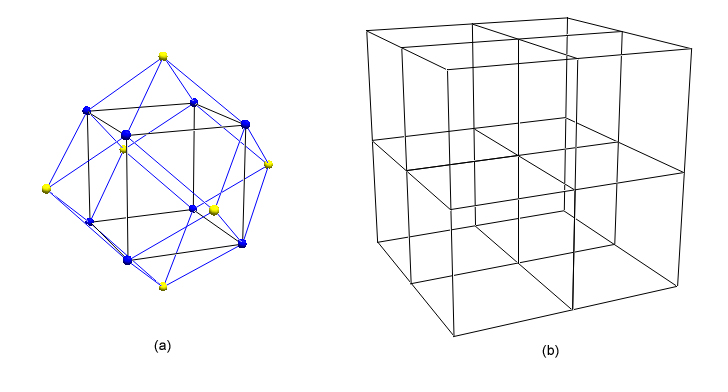
\includegraphics[scale=0.37,angle=0]{../img/initialGraphAndGrid.jpg}
    \caption{Initial mesh and its associated graph.}
    \label{FIG_INITIAL_GRAPH_MESH}
\end{figure}


Associated to this initial division of the unit cube into eight
equal cubic cells is an initial graph (Figure
\ref{FIG_INITIAL_GRAPH_MESH}(a)). To each cell corresponds a
\textit{cell node} in the graph (dark colored in Figure
\ref{FIG_INITIAL_GRAPH_MESH}(a)). Each cell node stores any
information associated to the cell it represents in variables, such
as the spatial coordinates of its centers and physical states (if
the numerical simulation of a physical phenomenon is intended; their
number varies according to the problem being considered). Each of
the eight cell nodes in Figure \ref{FIG_INITIAL_GRAPH_MESH}(a) has
six links oriented along the six directions: \textit{east}, along
positive $y$ direction; \textit{west}, along negative $y$ direction;
\textit{north}, along positive $z$ direction; \textit{south}, along
negative $z$ direction; \textit{front}, along positive $x$
direction, and \textit{back}, along negative $x$ direction. In the
computer code, these six links are six pointers.

Each cell node has also two special pointers called \textit{next}
and \textit{previous}. These pointers are used for ordering the cell
nodes in the graph. Since the graph can become very irregular after
successive refinements of different depths in different regions of
the domain, it can become very difficult to visit the cells in a
systematic way. This auxiliary chain list facilitates the access to
the graph cell nodes, independently of any topological configuration
the graph may assume. The maintenance of this list and the
definition of the order of each cell node in it is done by the
Hilbert curve, as will be explained in detail in Section
\ref{SEC_HILBERT_CURVE}.

The cell nodes also possess a variable that stores its current
refinement level. When a cell node of level $n$ is refined, its
eight daughter cells will each have level $n+1$. After a
derefinement, the opposite happens: eight cells of level $n$ fuse in
order to constitute a cell of level $n-1$.

In the graph structure underlying ALG there is another type of node
called a \textit{transition node}, which is used to connect cell
nodes of different refinement levels. Each transition node has five
links: one single connector and four quadruple connectors. These
five links are implemented as five pointers in the computer code.
They too are assigned variables corresponding to their refinement
levels. In order to better understand the purpose of these
transition nodes, consider the graph in Figure
\ref{FIG_REFINED_GRAPH}, which has a bunch of eight cells with one
level of refinement higher than the refinement level of the initial
cells.

%INITIAL GRAPH
\begin{figure}[H]
    \centering
    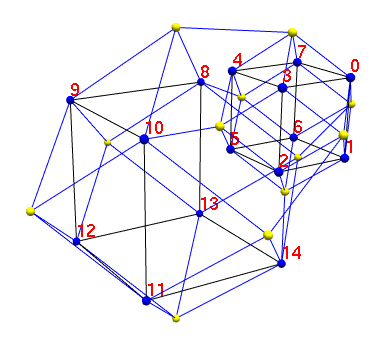
\includegraphics[scale=0.6,angle=0]{../img/refinedGraph.jpg}
    \caption{Communication between cell nodes and transition nodes.}
    \label{FIG_REFINED_GRAPH}
\end{figure}

Cell nodes $2$, $3$, $4$ and $5$ have cell node $10$ as the neighbor
in the west direction. Reciprocally, cell node $10$ has cell nodes
$2$, $3$, $4$ and $5$ as its neighbors in the east direction. Cell
nodes $2$, $3$, $4$ and $5$ could point their respective west
pointers to cell node $10$, but there is no way cell node $10$ can
point its only east pointer to the four neighbor cells
simultaneously. For this reason, a transition node has been created
in order to handle the communication between these nodes. Thus, the
east pointer of cell node $10$ is pointed to the transition node,
whose four quadruple connectors points each to each of the four cell
nodes $2$, $3$, $4$ and $5$. The single connector of the transition
node is pointed to cell node $10$ and the west pointer of each of
the nodes $2$, $3$, $4$ and $5$ is pointed to the transition node.

\subsection{Implementation}
The implementation chosen in this paper is based on the
object-oriented programming paradigm. The class \textit{Cell}
represents the nodes of the graph, irrespective of their types.
Since there are two different types of nodes, two inherited classes
were created: class \textit{CellNode} represents the cell nodes and
class \textit{TransitionNode} represents the transition nodes. See
Figure \ref{FIG_CELL_DIAGRAM}.

%CLASSES Cell, CellNode e TransitionNode
\begin{figure}[H]
    \centering
    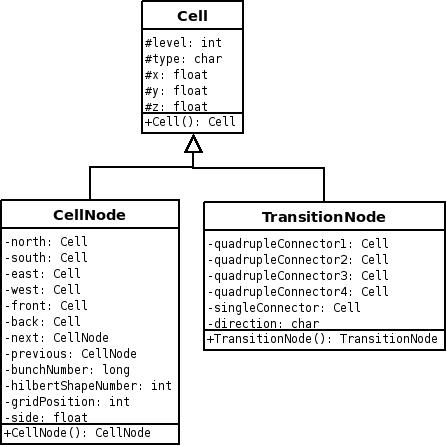
\includegraphics[scale=0.48,angle=0]{../img/cellDiagram.jpg}
    \caption{Hierarchy of classes Cell, CellNode and TransitionNode.}
    \label{FIG_CELL_DIAGRAM}
\end{figure}

The ALG graph itself is encapsulated by the class \textit{Grid}. The
refinement and derefinement methods, as well as other methods of
internal use for the maintenance of the data structure, are
implemented as members of this class (see Figure
\ref{FIG_GRID_DIAGRAM}).

%CLASS Grid
\begin{figure}[!ht]
    \centering
    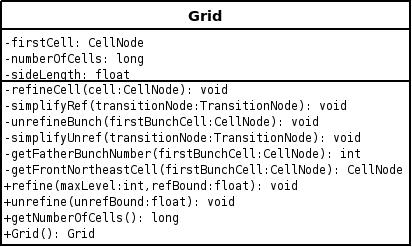
\includegraphics[scale=0.48,angle=0]{../img/gridDiagram.jpg}
    \caption{Class Grid.}
    \label{FIG_GRID_DIAGRAM}
\end{figure}

When an object of type \textit{Grid} is instantiated, the
constructor generates an initial graph as the one of Figure
\ref{FIG_INITIAL_GRAPH_MESH}. The steps necessary for the creation
of this initial graph are described by the algorithm
\ref{CONSTRUCTOR}.

\alglanguage{pseudocode}
\begin{algorithm}[!ht]
    \caption{Steps followed by the constructor of class Grid in order to create the initial graph.}
    \small{
    \begin{algorithmic}[1]
            \State Create eight cell nodes.
            \State Create six transition nodes.
            \State $sideLength \gets 1$

            \State
            \For{\textbf{each} cell node}
                \State Compute and set current node's coordinates.
                \State Points each current node's directional pointers to appropriate cell.
                \State Set current node's previous and next pointers according to Hilbert curve's ordering.
                \State Set current node's level to one.
                \State Set current node's side to $sideLength / 2$.
                \State Initialize other attributes pertinent to the current application.
            \EndFor

            \State
            \For{\textbf{each} transition node}
                \State Compute and set current node's coordinates.
                \State Point each current node's quadruple connector to appropriate cell node.
                \State Set current node's single connector to null.
                \State Set current node's level to one.
            \EndFor

            \State
            \State $numberOfCells \gets 8$.
            \State Set pointer $firstCell$ to the first cell of the Hilbert Curve list.
    \end{algorithmic} \label{CONSTRUCTOR}
    }
\end{algorithm}

The remaining members of class \textit{Grid}, which perform the
functions of refinement, derefinement and ordering of the cell nodes
via the Hilbert curve, will be discussed in the next sections.

    \section{Refinement}  \label{SEC_REFINEMENT}
The operation of \textit{refining} a cell is defined as dividing it
into eight equal cubic cells. When a cell is refined, the cell node
which represents it in the graph structure is replaced by a
structure consisting of eight cell nodes and six transition nodes,
which is similar to the initial graph. In order to exemplify the
refinement process, consider the refinement of cell number $0$ in
the mesh of Figure \ref{FIG_MESH_REFINEMENT}(a).

%FIG_MESH_REFINEMENT
\begin{figure}[!ht]
    \centering
    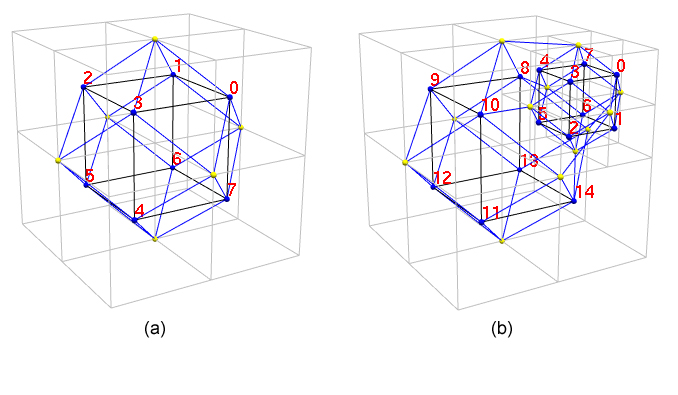
\includegraphics[scale=0.45,angle=0]{../img/gridAndGraph.jpg}
    \caption{Refinement of one cell.}
    \label{FIG_MESH_REFINEMENT}
\end{figure}

\noindent After refinement, cell $0$ will be divided into eight
smaller cells, half the length of the original one, with centers

\[
  \left(\frac{7}{8},\frac{7}{8},\frac{7}{8}\right),
  \left(\frac{7}{8},\frac{7}{8},\frac{5}{8}\right),
  \left(\frac{7}{8},\frac{5}{8},\frac{5}{8}\right),
  \left(\frac{7}{8},\frac{5}{8},\frac{7}{8}\right),
\]

\[
  \left(\frac{5}{8},\frac{7}{8},\frac{7}{8}\right),
  \left(\frac{5}{8},\frac{7}{8},\frac{5}{8}\right),
  \left(\frac{5}{8},\frac{5}{8},\frac{5}{8}\right),
  \left(\frac{5}{8},\frac{5}{8},\frac{7}{8}\right),
\]
resulting in the mesh of Figure \ref{FIG_MESH_REFINEMENT}(b).

More generally, when a cell centered at $(a, b, c)$ and length $L$
is refined, it is replaced by eight cells with length $L/2$ and
centers
\[
\left(a-\frac{L}{4},b-\frac{L}{4},c-\frac{L}{4}\right),
\left(a+\frac{L}{4},b-\frac{L}{4},c-\frac{L}{4}\right),
\left(a-\frac{L}{4},b+\frac{L}{4},c-\frac{L}{4}\right),
\]
\[
\left(a-\frac{L}{4},b-\frac{L}{4},c+\frac{L}{4}\right),
\left(a+\frac{L}{4},b+\frac{L}{4},c-\frac{L}{4}\right),
\left(a+\frac{L}{4},b-\frac{L}{4},c+\frac{L}{4}\right),
\]
\[
\left(a-\frac{L}{4},b+\frac{L}{4},c+\frac{L}{4}\right),
\left(a+\frac{L}{4},b+\frac{L}{4},c+\frac{L}{4}\right).
\]

The group of eight cells arising from a single original cell through
refinement will be called a \textit{bunch}. The cells of the new
bunch are ordered by the modified Hilbert curve, as will be
explained in Section \ref{SEC_HILBERT_CURVE}. The creation and
ordering of the new bunch of cells is merely a local event, which
alters only the states of the neighboring cells of the original
cell. These neighbor cells accordingly need to be notified of the
local change in the graph structure.

A cell that was just refined receives as its refinement level the level of the original unrefined cell plus one.
By convention, the cells of the initial mesh possess refinement
levels equal to $1$. In Figure \ref{FIG_MESH_REFINEMENT}(b), for
instance, cells number $0$ to $7$ have refinement level $2$, while
the remaining cells possess refinement level $1$. Transition nodes
are also assigned refinement levels, equal to the refinement levels
of the cells of the bunch in which they were created.

The length of a cubic cell $L$ relates to its refinement level $n$
through the simple relation

\begin{equation} \label{EQ_EDGE_SIZE}
 L = \frac{1}{2^n}.
\end{equation}

\subsection{Mesh refinement}
Mesh refinement is done according to criteria laid out by the
specific application. In the typical setting of adaptive mesh
refinement (AMR), when the variation of some physical variable in
the cells within a region of the computational domain exceeds some
preset value, called here the \textit{refinement bound}, indicating
that more precision might be needed in order to obtain more accurate
results, the program decides that the cells belonging to that region
must be refined. The program traverses the entire mesh in each
global iteration of the computations, verifying if any cell
satisfies the refinement condition defined by the application. When
a visited cell satisfies the condition, it is refined, originating a
modified mesh and its associated graph for the next global iteration
of the program.

Algorithm \ref{REFINEMENT_PROCEDURE} describes function
\textit{refine()}, which is responsible for the mesh refinement. It
receives as parameters the \textit{minimum refinement level} desired
for the mesh's cells, which is related to the minimum mesh size
initially expected necessary in order to get a reasonably meaningful
approximation to the solution of the problem being studied, and the
refinement bound discussed above.

\alglanguage{pseudocode}
\begin{algorithm}[!ht]
    \caption{Mesh refinement}
    \small{
    \begin{algorithmic}[1]
    \Procedure{refine}{minLevel, refinementBound}
        \State $CellNode \hspace{2mm} currentCell$
        \State $CellNode \hspace{2mm} auxiliar$
        \State $continueRefining \gets true$
        \While{$continueRefining$}
            \State $currentCell \gets firstCell$
            \State $continueRefining \gets false$
            \While{$currentCell$ is not $null$}
                \If{$currentCell.level < minLevel$ \textbf{and} the local spatial variation of some
                property in the cell exceeds the refinement bound}
                    \State $auxiliar \gets currentCell$
                    \State $currentCell \gets currentCell.next $
                    \State $refineCell(auxiliar)$
                    \State $numberOfCells \gets numberOfCells + 7$
                    \State $continueRefining \gets true$
                \Else
                    \State$currentCell \gets currentCell.next$
                \EndIf
            \EndWhile
        \EndWhile
    \EndProcedure
    \end{algorithmic}
    }
    \label{REFINEMENT_PROCEDURE}
\end{algorithm}

Notice in Algorithm \ref{REFINEMENT_PROCEDURE} that the attribute
that stores the number of cell nodes increases by $7$ at each cell
refinement and not by $8$. This happens because the cell node which
originated the new bunch is not stored as it would be in a typical
tree structure, but is completely replaced by the new bunch.
Moreover, in order to augment the performance, the cell node is not
actually destroyed upon refinement but is transformed into part of
the new bunch (specifically, it becomes the front northeast cell
node, as will be explained in the following). Thus, only $7$ new
cell nodes are created when a cell is refined.

\subsection{Cell refinement} \label{SUBSEC_PROCEDURE_REF}
The refinement of one cell is done by the function
\textit{refineCell()}. The process occurs in seven steps as
described below. Each step will be presented afterwards in a
detailed algorithm.

\begin{enumerate}
 \item Transformation of the cell to be refined into the front northeast cell of the new
 bunch.
 \item Creation of the remaining 7 cell nodes of the new bunch.
 \item Creation of 6 transition nodes.
 \item Linking of the cell and transition nodes of the new bunch.
 \item Linking of the neighboring cells of the original cell to the transition nodes of the new
 bunch.
 \item Ordering of the cells of the new bunch using the modified
 Hilbert curve.
 \item Elimination of unnecessary transition nodes.
\end{enumerate}

\subsubsection*{Step 1. Creation of the front northeast cell of new bunch}
In step 1, the cell to be refined becomes the front northeast cell
of the new bunch. Its attributes, such as geometric coordinates,
refinement level and others which depend on the problem being
considered, are accordingly updated at this stage, as described in
Algorithm \ref{STEP_1_REFINEMENT}.

\alglanguage{pseudocode}
\begin{algorithm}
    \caption{Step 1 of 7}
    \small{
    \begin{algorithmic}[1]
        \Procedure{refineCell}{cellNode}
        \State $fatherBunchNumber \gets cellNode.bunchNumber$
        \State $CellNode \hspace{2mm} frontNE \gets cellNode$
        \State $frontNE.level \gets cellNode.level + 1$
        \State $frontNE.side \gets cellNode.side / 2$
        \State $frontNE.x \gets cellNode.x + cellNode.side / 4$
        \State $frontNE.y \gets cellNode.y + cellNode.side / 4$
        \State $frontNE.z \gets cellNode.z + cellNode.side / 4$
        \State $frontNE.bunchNumber \gets fatherBunchNumber*10 + 1$
        \algstore{refinement}
    \end{algorithmic}
    }
    \label{STEP_1_REFINEMENT}
\end{algorithm}
\noindent The meaning of the attributes \textit{bunchNumber} and
\textit{fatherBunchNumber} will be explained in the next step.

\subsubsection*{Step 2. Creation of the remaining cells of the new bunch} \label{SUBSEC_REFINEMENT_STEP2}
In this step, the remaining seven cells of the bunch with all their
attributes are created, as described in Algorithm
\ref{STEP_2_REFINEMENT}.

\alglanguage{pseudocode}
\begin{algorithm}[!h]
    \caption{Step 2 of 7}
    \small{
    \begin{algorithmic}[1]
        \algrestore{refinement}
        \State $CellNode \hspace{2mm} backNE \gets \New \hspace{2mm} CellNode$
        \Comment{Back northeast cell.}

        \State $CellNode \hspace{2mm} backNW \gets \New \hspace{2mm} CellNode$
        \Comment{Back northwest cell.}

        \State $CellNode \hspace{2mm} frontNW \gets \New \hspace{2mm} CellNode$
        \Comment{Front northwest cell.}

        \State $CellNode \hspace{2mm} frontSW \gets \New \hspace{2mm} CellNode$
        \Comment{Front southwest cell.}

        \State $CellNode \hspace{2mm} backSW \gets \New \hspace{2mm} CellNode$
        \Comment{Back southwest cell.}

        \State $CellNode \hspace{2mm} backSE \gets \New \hspace{2mm} CellNode$
        \Comment{Back southeast cell.}

        \State $CellNode \hspace{2mm} frontSW \gets \New \hspace{2mm} CellNode$
        \Comment{Front southwest cell.}

        \State
        \For{\textbf{each} new cell}
            \State sets current cell's level to $frontNE.level$
            \State sets current cell's side length to $frontNE.side$
            \State computes and sets current cell's coordinates
            \State computes and sets other attributes of current
            cell
        \EndFor

        \State
        \State $backNE.bunchNumber \gets fatherBunchNumber*10 + 2$
        \State $backNW.bunchNumber \gets fatherBunchNumber*10 + 3$
        \State $frontNW.bunchNumber \gets fatherBunchNumber*10 + 4$
        \State $frontSW.bunchNumber \gets fatherBunchNumber*10 + 5$
        \State $backSW.bunchNumber \gets fatherBunchNumber*10 + 6$
        \State $backSE.bunchNumber \gets fatherBunchNumber*10 + 7$
        \State $frontSW.bunchNumber \gets fatherBunchNumber*10 + 8$
        \algstore{refinement}
    \end{algorithmic}
    }
    \label{STEP_2_REFINEMENT}
\end{algorithm}

In the derefinement process, those cells which originated from the
same cell (i.e., cells that belong to the same bunch) must again
become one cell, with some of the attributes of the original cell
being restored. In order to easily identify the original cell, even
after undergoing several steps of refinement, it is necessary that
each cell stores information regarding the cell which originated it.
This identification process is carried out through specific
modifications of the identifier \textit{bunchNumber} of each cell at
each refinement step. This attribute identifies each cell uniquely
and stores information about its origin.

At each refinement step, the attribute \textit{bunchNumber} of each
cell of the new bunch is initially configured to be the
\textit{bunchNumber} of the cell being refined multiplied by 10,
which corresponds to shifting one unit to the left the numerals of
\textit{bunchNumber} of the original cell. Since this identifier
must be unique, a different numeral between 1 and 8 is then added to
the result for each cell of the bunch.

Therefore, in order to identify the \textit{bunchNumber} of the
originating cell of any cell node of the graph, it suffices to
divide the \textit{bunchNumber} of the cell node by 10 and discard
the remainder. Any cell node which belongs to the same bunch will
produce the same number. Thus, the derefinement procedure will
easily be able to identify when two cells belong to the same bunch.


\subsubsection*{Step 3. Creation of transition nodes of the new bunch}
In order to complete the set of nodes of the new bunch, six
transition nodes must be created. They are responsible for linking
the bunch to the neighboring cells of the cell just refined, that
is, link the new bunch to the graph. This stage is described by
Algorithm \ref{STEP_3_REFINEMENT}.

\alglanguage{pseudocode}
\begin{algorithm}[!hb]
    \caption{Step 3 of 7}
    \small{
    \begin{algorithmic}[1]
        \algrestore{refinement}
        \State $TransitionNode \hspace{2mm} northTN \gets \New \hspace{2mm} TransitionNode$
        \Comment{North transition node.}

        \State $TransitionNode \hspace{2mm} southTN \gets \New \hspace{2mm} TransitionNode$
        \Comment{South transition node.}

        \State $TransitionNode \hspace{2mm} eastTN \gets \New \hspace{2mm} TransitionNode$
        \Comment{ East transition node}.

        \State $TransitionNode \hspace{2mm} westTN \gets \New \hspace{2mm} TransitionNode$
        \Comment{ West transition node.}

        \State $TransitionNode \hspace{2mm} frontTN \gets \New \hspace{2mm} TransitionNode$
        \Comment{Front transition node.}

        \State $TransitionNode \hspace{2mm} backTN \gets \New \hspace{2mm} TransitionNode$
        \Comment{ Back transition node.}


        \State $ $
        \For{\textbf{each} new transition node}
            \State sets current node's level to $frontNE.level$
            \State computes and sets current node's coordinates
            \State points current node's single connector to appropriate cellNode's neighbor
        \EndFor
        \algstore{refinement}
    \end{algorithmic}
    }
    \label{STEP_3_REFINEMENT}
\end{algorithm}
At line 42 of Algorithm \ref{STEP_3_REFINEMENT} the single connector
of the transition node is pointed to the neighbor cell of
\textit{cellNode} (the refined cell) which is in the same direction
as the transition node itself. For instance, north transition node
points its single connector to the neighbor cell of
\textit{cellNode} which is pointed at by the pointer of
\textit{cellNode} in the direction \textit{north}. The same happens
to the remaining nodes, so that in the end of the loop all
transition nodes are appropriately connected to the neighboring
cells of the refined cell. Although transition nodes need not be
assigned geometrical coordinates (since they do not exist physically
in the computational domain), they are assigned coordinates for the
purpose of drawing the graph if one so wishes.

In order to complete the two-directional link between nodes, there
remains to point the node which was pointed to by the transition
node to the transition node itself. In the example of the previous
paragraph, if the node pointed to is a cell node, its pointer of
direction \textit{south} must be pointed to transition node
\textit{north}. If the node is a transition node, one of its
quadruple connectors or its single connector must be pointed to
transition node \textit{north}. The verification of node type and
the determination of the type of connector is done at step 5.


\subsubsection*{Step 4. Linking of cell and transition nodes}
After the creation and initialization of cell and transition nodes
of the new bunch, these must be linked, forming a structure as shown
in Figure \ref{FIG_BUNCH}.  These linkings are done by Algorithm
\ref{STEP_4_REFINEMENT}.

%FIG_BUNCH
\begin{figure}[ht]
    \centering
    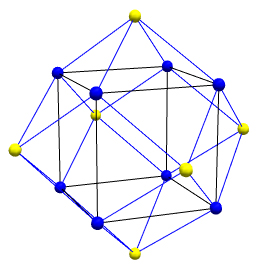
\includegraphics[scale=0.35]{../img/bunch.jpg}
    \caption{Linking between cell and transition nodes.}
    \label{FIG_BUNCH}
\end{figure}

\alglanguage{pseudocode}
\begin{algorithm}[h]
    \caption{Step 4 of 7}
    \small{
    \begin{algorithmic}[1]
        \algrestore{refinement}
        \For{\textbf{each} cell node}
            \State updates each current cell's direction pointer
        \EndFor
        \State
        \For{\textbf{each} transition node}
            \State updates each current node's quadruple connector
        \EndFor
        \algstore{refinement}
    \end{algorithmic}
    }
    \label{STEP_4_REFINEMENT}
\end{algorithm}

The first loop of Algorithm \ref{STEP_4_REFINEMENT} configures the
directional pointers of each cell node in the bunch. For instance,
pointer \textit{north} of front northeast cell is pointed to the
north transition node, while pointer \textit{south} is pointed to
the front southeast cell node. At the end of the loop, all
directional pointers of all cell nodes will be appropriately
configured.

The second loop configures the quadruple connectors of the
transition nodes. A scheme is defined to determine to which cell
each quadruple connector must point. This must be done in a very
precise way, as this choice will interfere in the simplification
procedure. Figure \ref{SCHEME_4CONNECTORS} shows the adopted scheme.

\begin{figure}[!ht]
    \centering
    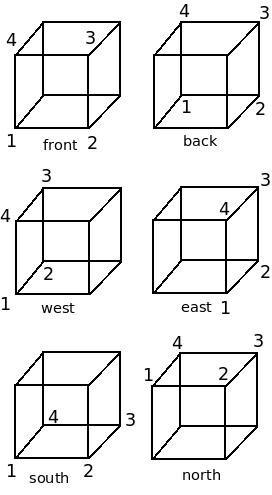
\includegraphics[scale=0.5]{../img/order_4connectors.jpg}
    \caption{Configuration scheme for quadruple connectors of the transition nodes.}
    \label{SCHEME_4CONNECTORS}
\end{figure}

For instance, as seen in the second cube in the second column of
Figure \ref{SCHEME_4CONNECTORS}, quadruple connectors 1, 2, 3 and 4
of transition node (\textit{east}) are respectively pointed to node
cells front southeast, back southeast, back northeast and front
northeast.


\subsubsection*{Step 5. Linking of the graph to the new bunch}
In step 3, after being created, the transition nodes of the new
bunch were pointed to the neighboring cells of the just refined
\textit{cellNode} thereby linking it to the graph of the mesh.
Reciprocally, the graph itself must be connected to the new bunch,
since all links in the graph are bidirectional; at this point in the
algorithm the neighboring nodes of the refined cell still point to
\textit{cellNode}, which no longer exists. This update is done by
Algorithm \ref{STEP_5_REFINEMENT}, where the neighboring nodes to
the refined cell are linked to the six transition nodes of the
bunch.

\alglanguage{pseudocode}
\begin{algorithm}[!hb]
    \caption{Step 5 of 7}
    \small{
    \begin{algorithmic}[1]
        \algrestore{refinement}
        \State $char$ $direction$
        \State $CellNode$  $neighborCN$
        \State $TransitionNode$  $neighborTN$
        \State $TransitionNode$ $transitionNode[6]$
        \State $transitionNode[0] \gets northTN$
        \State $transitionNode[1] \gets southTN$
        \State $transitionNode[2] \gets eastTN$
        \State $transitionNode[3] \gets westTN$
        \State $transitionNode[4] \gets frontTN$
        \State $transitionNode[5] \gets backTN$
        \State
        \For{i $\gets$ 0 \textbf{to} 5}
            \If{$transitionNode[i]\cdot singleConnector$ is a cell node}
                \State $neighborCN \gets transitionNode[i].singleConnector$
                \State $direction \gets transitionNode[i].direction$
                \State $neighborCN.oppositeDirection(direction) \gets transitionNode[i]$

            \Else \Comment{In this case the neighboring cell is a transition node}
                \State $neighborTN \gets transitionNode[i].singleConnector$
                \If{$neighborTN.singleConnector == cellNode$}
                    \State $neighborTN.singleConnector \gets transitionNode[i]$
                    \State
                \ElsIf{$neighborTN.quadrupleConnector1 == cellNode$}
                    \State $neighborTN.quadrupleConnector1 \gets transitionNode[i]$
                    \State
                \ElsIf{$neighborTN.quadrupleConnector2 == cellNode$}
                    \State $neighborTN.quadrupleConnector2 \gets transitionNode[i]$
                    \State
                \ElsIf{$neighborTN.quadrupleConnector3 == cellNode$}
                    \State $neighborTN.quadrupleConnector3 \gets transitionNode[i]$
                    \State
                \ElsIf{$neighborTN.quadrupleConnector4 == cellNode$}
                    \State $neighborTN.quadrupleConnector4 \gets transitionNode[i]$

                \Else
                    \State $print('Error')$
                \EndIf
            \EndIf
        \EndFor
        \algstore{refinement}
    \end{algorithmic}
    }
    \label{STEP_5_REFINEMENT}
\end{algorithm}

The neighboring nodes of the refined cell \textit{cellNode} can be
either cell nodes or transition nodes. When the neighbor node is a
cell node, the directional pointer of that node must be pointed to
the transition node whose direction is opposite to that of the
transition node. For example, assume that the north transition node
has a cell node as a neighbor, that is, its single connector points
to a cell node. This neighboring cell node must have its directional
pointer \textit{south} pointed to the north transition node. In
Algorithm \ref{STEP_5_REFINEMENT}, this task is executed in line 66,
where method \textit{oppositeDirection()} returns the directional
pointer whose direction is opposite to that received as a parameter.

In case the neighboring node of the transition node of the bunch is
also a transition node, then an analysis of its single connector and
all its quadruple connectors must be done in order to determine
which one points to \textit{cellNode}, which is the one who must be
updated and pointed to the transition node of the bunch. This
analysis and update are done by the piece of code between lines 67
and 86.

\subsubsection*{Step 6. Ordering of the cell nodes of the graph using the modified Hilbert curve}
The modified Hilbert curve is a space filling curve which is capable
of passing through all the points of a three-dimensional mesh
irrespective of how irregular this mesh might be. Its implementation
is done by means of a double chain list where each cell node
possesses two additional pointers: \textit{next} and
\textit{previous}. Any cell of the mesh can be reached traversing
the chain list defined by the Hilbert curve to the point it
occupies.

When a cell is refined, the 8 new cells of the bunch must be ordered
and inserted in the Hilbert curve, in order to be accessible later.
They are ordered in a small list, according to the relative position
of the refined cell in the Hilbert curve of the graph (before
refinement), which is later inserted in the main list. This
preordering in a sublist guarantees that the cells of the same bunch
will always be near each other in the ordering of the curve, causing
only a local modification in the curve. Therefore, inserting the new
cells in the main curve consists only in inserting an already
ordered sublist in the position of the cell just refined. The manner
in which this is done is detailed in Section
\ref{SEC_HILBERT_CURVE}. However, the implementation is done at this
step of the refinement, where the references for the pointers
\textit{next} and \textit{previous} of each cell of the bunch are
defined. Algorithm \ref{STEP_6_REFINEMENT} shows how this is
executed.

\alglanguage{pseudocode}
\begin{algorithm}[!ht]
    \caption{Step 6 of 7}
    \small{
    \begin{algorithmic}[1]
        \algrestore{refinement}
        \For{\textbf{each} cell node}
            \State sets current cell's next pointer according to modified Hilbert curve algorithm
            \State sets current cell's previous pointer according to modified Hilbert curve algorithm
        \EndFor
        \algstore{refinement}
    \end{algorithmic}
    }
    \label{STEP_6_REFINEMENT}
\end{algorithm}


\subsubsection*{Step 7. Removal of unnecessary transition nodes of the graph}
The function of the transition nodes in the ALG data structure is to
enable the communication between nodes of different levels of
refinement. In the refinement process, transition nodes are created
to connect the cells of the new bunch with the neighboring cells of
the refined cell. However, the neighborhood of the refined cell may
contain cells which have the same level of refinement of the cells
of the new bunch. In this situation a transition node is
dispensable, since the cells can be directly linked.

For instance, in Figure \ref{FIG_BEFORE_SIMPLIFY}, we have two
neighboring bunches whose cell nodes possess the same refinement
levels and which are connected by means of two transition nodes.
However, they can be directly connected as shown in Figure
\ref{FIG_AFTER_SIMPLIFY}.

%WITHOUT SIMPLIFICATION
\begin{figure}[!ht]
    \centering
    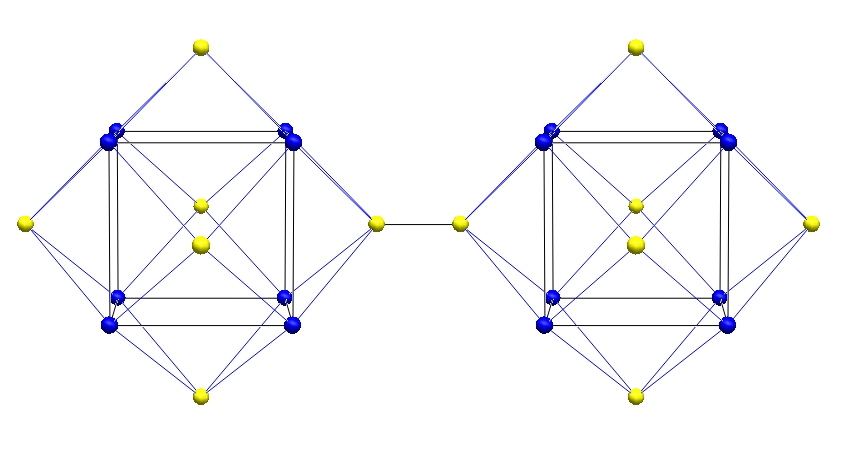
\includegraphics[scale=0.20,angle=0]{../img/graphNotSimplified.jpg}
    \caption{Graph before simplification showing two unnecessary transition nodes.}
    \label{FIG_BEFORE_SIMPLIFY}
\end{figure}


%WITH SIMPLIFICATION
\begin{figure}[!ht]
    \centering
    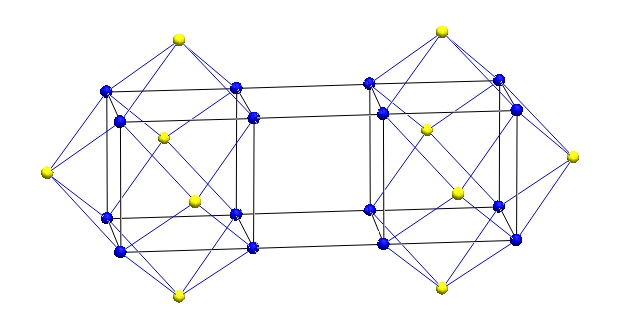
\includegraphics[scale=0.3,angle=0]{../img/graphSimplified.jpg}
    \caption{Simplified graph with transition nodes eliminated and cell nodes directly linked.}
    \label{FIG_AFTER_SIMPLIFY}
\end{figure}

In order to eliminate the storage problem associated with keeping
unnecessary transition nodes, the last step in the refinement
process contains a \textit{simplification} procedure that deletes
needless transition nodes in the new bunch and its immediate
neighborhood, as well as makes the direct link between nodes with
the same refinement level. This procedure is detailed in the next
subsection.

\alglanguage{pseudocode}
\begin{algorithm}[!ht]
    \caption{Step 7 of 7}
    \small{
    \begin{algorithmic}[1]
        \algrestore{refinement}
        \For{i $\gets$ 0 \textbf{to} 5}
            \State $simplifyRef(transitionNode[i])$
        \EndFor
        \EndProcedure
    \end{algorithmic}
    }
    \label{STEP_7_REFINEMENT}
\end{algorithm}


\subsection{Simplification routine} \label{SUBSEC_SIMPLIFICATION_REF}

The simplification routine is executed by the code described in
Algorithm \ref{SIMPLIFICATION_REFINEMENT}. In order for a
simplification to occur, two conditions must be satisfied. The first
one is that the single connector of a transition node received as a
parameter in function \textit{simplifyRef()} must point to a
transition node. The second condition is that they must possess the
same refinement level. In Algorithm
\ref{SIMPLIFICATION_REFINEMENT} these conditions are verified
in lines 2 and 3.

\alglanguage{pseudocode}
\begin{algorithm}[!hb]
    \caption{Simplification - Refinement}
    \small{
    \begin{algorithmic}[1]
    \Procedure{simplifyRef}{transitionNode}
    \If{$transitionNode.singleConnector.type == transitionNode.type$}
        \If{$transitionNode.singleConnector.level == transitionNode.level$}
            \State
            \State $TransitionNode$ $neighborTN \gets transitionNode.singleConnector$
            \State $char$ $dir \gets neighTN.direction$
            \State $CellNode$ $quadCon[4]$ \Comment{Stores the node's quadruple connectors}
            \State $Cell$ $nQuadCon[4]$ \Comment{Stores the neighbor node's quadruple connectors}
            \State
            \State $quadCon[0] \gets transitionNode.quadrupleConnector1$
            \State $quadCon[1] \gets transitionNode.quadrupleConnector2$
            \State $quadCon[2] \gets transitionNode.quadrupleConnector3$
            \State $quadCon[3] \gets transitionNode.quadrupleConnector4$
            \State
            \State $nQuadCon[0] \gets neighborTN.quadrupleConnector1$
            \State $nQuadCon[1] \gets neighborTN.quadrupleConnector2$
            \State $nQuadCon[2] \gets neighborTN.quadrupleConnector3$
            \State $nQuadCon[3] \gets neighborTN.quadrupleConnector4$

            \State
            \For{$i \gets 0$ \textbf{to} $3$}
                \State $quadCon[i].oppositeDirection(dir) \gets nQuadCon[i]$
            \EndFor
            \State $dir \gets transitionNode.direction$
            \For{$i \gets 0$ \textbf{to} $3$}
                \If{$nQuadCon[i]$ is a cell node}
                    \State $nQuadCon[i].oppositeDirection(dir) \gets quadCon[i]$
                \Else

                    \If{$neighborTN == nQuadCon[i].singleConnector$}
                        \State $nQuadCon[i].singleConnector \gets quadCon[i]$
                    \ElsIf{$neighborTN == nQuadCon[i].quadrupleConnector1$}
                        \State $nQuadCon[i].quadrupleConnector1 \gets quadCon[i]$
                    \ElsIf{$neighborTN == nQuadCon[i].quadrupleConnector2$}
                        \State $nQuadCon[i].quadrupleConnector2 \gets quadCon[i]$
                    \ElsIf{$neighborTN == nQuadCon[i].quadrupleConnector3$}
                        \State $nQuadCon[i].quadrupleConnector3 \gets quadCon[i]$
                    \ElsIf{$neighborTN == nQuadCon[i].quadrupleConnector4$}
                        \State $nQuadCon[i].quadrupleConnector4 \gets quadCon[i]$
                    \Else
                        \State $print('Error')$
                    \EndIf
                \EndIf
            \EndFor
            \State
            \State \textbf{delete} $transitionNode$
            \State \textbf{delete} $neighborTN$
        \EndIf
    \EndIf
    \EndProcedure
    \end{algorithmic}
    }
    \label{SIMPLIFICATION_REFINEMENT}
\end{algorithm}

When both conditions are obeyed, the graph must be simplified.
Before removing the unnecessary transition nodes, the references of
their quadruple connectors must be stored, since they are the
references for the cell nodes which will be directly linked.

In Algorithm \ref{SIMPLIFICATION_REFINEMENT}, vector \textit{quadCon}
stores references for the quadruple connectors of the transition
node (\textit{transitionNode}) received as a parameter; vector
\textit{nQuadCon} stores references for the quadruple connectors of
the neighbor transition node (\textit{neighborTN}) which is pointed
to by the single connector of \textit{transitionNode}.

Thereafter, the cells of the bunch which are referenced by the
quadruple connectors of \textit{transitionNode} are pointed to those
referenced by the quadruple connectors of \textit{neighborTN}. This
is done by the loop between lines 20 and 22. The directional pointer
of each one of these nodes that must be reconfigured is the one
whose direction is opposite of that of \textit{neighborTN}. For
instance, assume in Figure \ref{FIG_BEFORE_SIMPLIFY} that the west
transition node of the right-hand bunch is passed as a parameter to
the simplification routine. Then the nodes which are referenced by
its quadruple connectors will point their \textit{west} directional
pointers to the nodes referenced by the quadruples connectors of the
east transition node of the left-hand side bunch. Here the scheme
depicted in Figure \ref{SCHEME_4CONNECTORS} guarantees that the
connections are correctly done.

Next the cells of the bunch which are referenced by the quadruple
connectors of \textit{neighborTN} are pointed to those referenced by
the quadruple connectors of \textit{transitionNode}. These nodes can
be either cell nodes or transition nodes. If they are cell nodes,
the directional pointer that must be reconfigured is that with
direction opposite to the one of \textit{transitionNode}. This is
done in line 26 of Algorithm \ref{SIMPLIFICATION_REFINEMENT}.
If they are transition nodes, one must first find out which type of
connector of these nodes points to \textit{neighborTN}. This is done
by the piece of code between lines 27 and 45.

After all neighbor nodes with the same refinement levels are
connected, the transition nodes \textit{transitionNode} and
\textit{neighborTN} are removed from the graph.

    \section{Derefinement} \label{SEC_DEREFINEMENT}

Derefinement means the fusion of eight cells with the same level of
refinement $n$ and belonging to the same bunch back into a unique
cell of refinement level $n - 1$ (Figures
\ref{FIG_BEFORE_DEREFINEMENT} and \ref{FIG_AFTER_DEREFINEMENT}).

\begin{figure}[H]
    \centering
    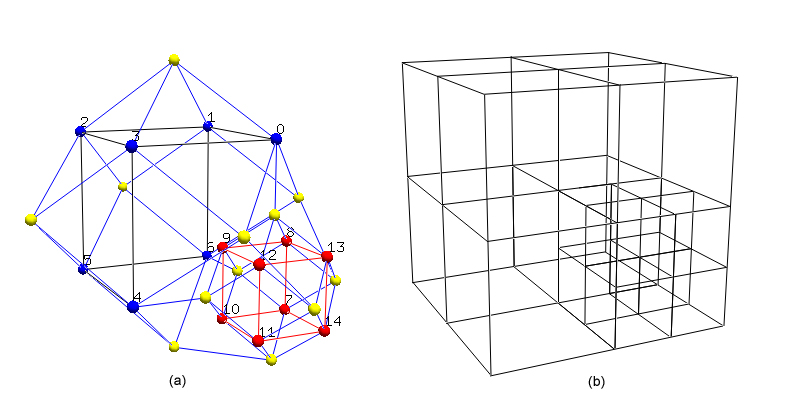
\includegraphics[scale=0.40]{../img/refinedGraphAndGrid.jpg}
    \caption{Graph and mesh before derefinement.}
    \label{FIG_BEFORE_DEREFINEMENT}
\end{figure}

\begin{figure}
    \centering
    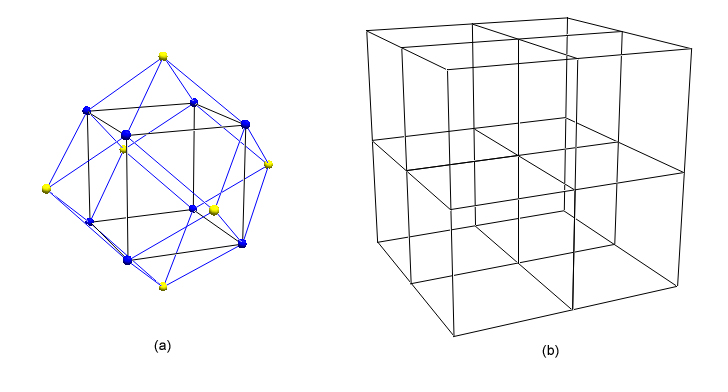
\includegraphics[scale=0.40]{../img/initialGraphAndGrid.jpg}
    \caption{Graph and mesh after derefinement.}
    \label{FIG_AFTER_DEREFINEMENT}
\end{figure}

The decision to derefine or not a bunch is taken according to
criteria established by the application. Generally, one derefines a
bunch when the variation in some physical variable within the cells
in a certain neighborhood is below some preset threshold. When this
happens, the number of cells in the region becomes greater than that
necessary in order to accomplish an accurate approximation of the
exact solution in that region, causing wastage of memory and
processing power.

\subsection{Mesh derefinement}
The derefinement of the mesh is done by the method
\textit{derefine()}. Whenever it is called upon, a research is done
on all cells of the mesh to determine which ones are qualified for
derefinement according to the criteria explained above.

Before a bunch is actually derefined, the cells initially qualified
for derefinement must pass some tests. First, all cells must belong
to the same bunch, otherwise it will not be allowed that the $8$
adjacent cells which define a cube in the mesh be derefined, even if
they satisfy the derefinement condition adopted by the application.
Second, all cells in the bunch must satisfy the derefinement
condition. Algorithm \ref{DEREFINEMENT_PROCEDURE} presented below
resumes what is done by method \textit{derefine()}. It receives as a
parameter the maximum variation accepted by one or more physical
variables upon which the derefinement is based.

\alglanguage{pseudocode}
\begin{algorithm}[!ht]
    \caption{Mesh derefinement}
    \small{
    \begin{algorithmic}[1]
    \Procedure{derefine}{maxPrecision}
        \State $CellNode \hspace{2mm} currentCell \gets firstCell$
        \State $CellNode \hspace{2mm} cellAfterBunch \gets currentCell$
        \While{$currentCell$ is not $null$}
            \If{$currentCell$ and its seven adjacent cells belong to the same bunch}
                \If{all cells of current bunch have the specified properties $>$ $maxPrecision$}
                    \State$cellAfterBunch \gets currentCell$
                    \For{i $\gets$ 0 \textbf{to} 8}
                         \State $cellAfterBunch \gets cellAfterBunch.next$
                     \EndFor
                    \State $derefineBunch(currentCell)$
                \EndIf
            \EndIf
            \State$currentCell \gets cellAfterBunch$
            \If{$cellAfterBunch$ is not $null$}
                \State$cellAfterBunch \gets cellAfterBunch.next$
            \EndIf
        \EndWhile
    \EndProcedure
    \end{algorithmic}
    }
    \label{DEREFINEMENT_PROCEDURE}
\end{algorithm}

Notice that in Line 5 the algorithm verifies if the current cell and
its seven adjacent cells belong to the same bunch. This happens when
they have the same refinement level and the division without
remainder of the attribute \textit{bunchNumber} of each cell wields
the same result.

Function \textit{derefineBunch()} called in Line 11 receives as a
parameter the first cell of the bunch to be refined. Its task is to
derefine the bunch, as will be discussed next.

\subsection{Bunch derefinement} \label{SUBSEC_PROCEDURE_DEREF}
The bunch derefinement procedure has as a parameter the first cell
of the bunch to be refined, as the mesh derefinement algorithm
encounters when it follows the ordering established by the Hilbert
curve. In order to obtain the remaining cells of the bunch, it just
follows the order given by the Hilbert curve until the seventh next
cell, because the Hilbert curve is built in such a way as to ensure
that all cells belonging to the same bunch follow in a sequence one
after the other in the chain list defined by the curve. Therefore,
is suffices to access the first cell of the list in order to obtain
access to the remaining cells of the bunch.

The entire process is divided below in six steps, each step
discussed in detail in the next paragraphs.

\begin{enumerate}
\item Creation of the cell node which will replace the bunch.
\item Creation of six transition nodes around the replacer cell node.
\item Linking between the cell and transition nodes just created.
\item Linking of the new transition nodes to the neighboring nodes of the bunch being derefined.
\item Elimination of all nodes of the bunch to be derefined.
\item Removal of unnecessary transition nodes in the neighborhood of the derefined bunch.
\end{enumerate}


\subsubsection*{Step 1. Creation of the cell node which replaces the bunch}
The derefinement procedure produces a cell with characteristics
which are similar to the cell which originated the bunch which is
being derefined. Its attributes are computed from the corresponding
attributes of the cells in the bunch. In the end, the group of eight
cells which form the bunch is replaced by the recently created cell.

In order to avoid the costs of memory allocation and management
associated with the creation of a new cell, one uses a preexistent
cell of the bunch to replace it. In this implementation, the front
northeast cell was chosen. Algorithm \ref{STEP_1_DEREFINEMENT}
(Lines 11 through 19) shows how this cell recovers some of the
geometric and topological attributes of the original cell that gave
origin to the bunch. Lines 12 through 14 reconfigure the geometric
coordinates. Line 15 computes the identifier of the replacer cell,
restoring it to the value of the cell which originated the bunch:
this identifier was built in such a way as to guarantee that all
cells belonging to the same bunch produce the same value when their
identifier is divided without remainder by 10 (see Step 2 in Section
\ref{SEC_REFINEMENT}). Line 16 computes the value of the basic form
of the Hilbert curve that will be attributed to the replacer cell;
this value is read by the refinement procedure, in case it is
decided in another iteration of the program that this cell must be
refined again, in order to tell how the cells of the resulting bunch
will be ordered by the Hilbert curve (see Section
\ref{SEC_HILBERT_CURVE}). This information is passed on by the cells
of the present bunch themselves, which give the replacer cell the
precise value so that in the future the cells of the newly refined
bunch should be ordered in the same way. This procedure is
fundamental for the correct functioning of the Hilbert curve. A call
to the function \textit{getFatherHilbertShape()} returns the number
of the Hilbert curve shape that was used in the refinement routine
for the ordering of the cells in the current bunch. Lines 17 and 18
update the refinement level and cell length, respectively. Other
variables which depend on the problem being considered should be
updated in this stage of the derefinement as well.

\alglanguage{pseudocode}
\begin{algorithm}[!ht]
    \caption{Step 1 of 6}
    \small{
    \begin{algorithmic}[1]
        \Procedure{derefineBunch}{firstBunchCell}
        \State $CellNode \hspace{2mm} frontNE \gets getFrontNortheastCell(firstBunchCell)$
        \State $CellNode \hspace{2mm} frontNW \gets frontNE.west$
        \State $CellNode \hspace{2mm} frontSE \gets frontNE.south$
        \State $CellNode \hspace{2mm} frontSW \gets frontNW.south$
        \State $CellNode \hspace{2mm} backNE \gets frontNE.back$
        \State $CellNode \hspace{2mm} backNW \gets backNE.west$
        \State $CellNode \hspace{2mm} backSE \gets backNE.south$
        \State $CellNode \hspace{2mm} backSW \gets backNW.south$
        \State
        \State $CellNode\hspace{2mm} replacerCell \gets frontNE$
        \State $replacerCell.x \gets (replacerCell.x + replacerCell.back.x) / 2$
        \State $replacerCell.y \gets (replacerCell.y + replacerCell.west.y) / 2$
        \State $replacerCell.z \gets (replacerCell.z + replacerCell.south.z) / 2$
        \State $replacerCell.bunchNumber \gets firstBunchCell.bunchNumber / 10$
        \State $replacerCell.HilbertShapeNumber \gets getFatherHilbertShape(firstBunchCell)$
        \State $replacerCell.level \gets firstBunchCell.level - 1$
        \State $replacerCell.side \gets cellNode.side * 2$
        \State updates other attributes.
        \State
        \State $CellNode\hspace{2mm} cellBeforeBunch \gets firstBunchCell.previous$
        \State $CellNode\hspace{2mm} cellAfterBunch \gets firstBunchCell$
        \For{i $\gets$ 0 \textbf{to} 8}
            \State $cellAfterBunch \gets cellAfterBunch.next$
        \EndFor
        \State $replacerCell.previous \gets cellBeforeBunch$
        \State $replacerCell.next \gets cellAfterBunch$
        \If{$replacerCell.previous$ is not null}
            \State $replacerCell.previous.next \gets replacerCell$
        \EndIf
        \If{$replacerCell.next$ is not null}
            \State $replacerCell.next.previous \gets replacerCell$
        \EndIf
        \algstore{derefinebunch}
    \end{algorithmic}
    }
    \label{STEP_1_DEREFINEMENT}
\end{algorithm}

It is necessary to store references for all cell nodes in the bunch.
This is done in Lines 2 through 9 in Algorithm
\ref{STEP_1_DEREFINEMENT}. In order to find out the front northeast
cell of the bunch, function \textit{getFrontNortheastCell()} is
called. Its determination is done analyzing the geometric
coordinates of all cells in the bunch.

The code from Lines 21 through 33 reconfigures the pointers
\textit{previous} and \textit{next} from the chain list defined by
the Hilbert curve. Since the cell nodes from the bunch will be
removed from the graph in the last stages of derefinement, it is
necessary that they be removed also from this chain list. The
removal action consists simply in substituting the replacer cell
node in place of the sublist of the bunch cells.

\subsubsection*{Step 2. Creation of the six transition nodes of the replacer cell node}
The replacer cell must have its directional pointers pointed to the
neighboring nodes of the bunch which is being derefined.  The
refinement level of these nodes may be different from the replacer
cell, making it necessary the existence of transition nodes for the
communication of nodes having different refinement levels. Therefore
a transition node is created for each direction. Notice that, if in
some direction the cells nodes have the same refinement level, no
transition node would be necessary in that direction. Nonetheless,
transition nodes are initially created in every direction; those
unneeded will be later removed in the simplification procedure (see
Step 6). Although in principle one could design the derefinement
procedure in such a way as not to create unnecessary transition
nodes from the start, this would unreasonably complicate matters,
making the algorithm difficult to understand and not gaining much in
terms of performance, since a simplifying procedure would be needed
anyway in order to get rid of unnecessary transition nodes present
in the neighborhood of the replaced bunch due to its neighboring
cells.

Figure \ref{FIG_DEREFINING} shows how the new transition nodes
(white circles) are related to the replacer cell and the replaced
bunch neighbors. The single connector of each node is pointed to the
replacer cell, while the quadruple connectors point to the
neighbors. Algorithm \ref{STEP_2_AND_3_DEREFINEMENT} shows how these
nodes are created. Note in Line 42 that the refinement level of each
transition node is configured to be one unit less than the
refinement level of the bunch, that is, to match the refinement
level of the replacer cell.


\begin{figure}[!hb]
    \centering
    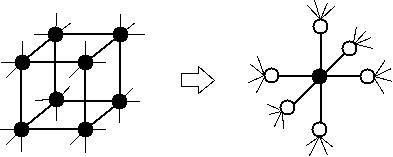
\includegraphics[scale=0.5]{../img/derefinement.jpg}
    \caption{Creation of transition nodes for the replacer cell.}
    \label{FIG_DEREFINING}
\end{figure}


\alglanguage{pseudocode}
\begin{algorithm}[!ht]
    \caption{Steps 2 and 3 of 6.}
    \small{
    \begin{algorithmic}[1]
        \algrestore{derefinebunch}
        \State $TransitionNode \hspace{2mm} northTN \gets \New \hspace{2mm} TransitionNode$
        \Comment{North node.}

        \State $TransitionNode \hspace{2mm} southTN \gets \New \hspace{2mm} TransitionNode$
        \Comment{South node.}

        \State $TransitionNode \hspace{2mm} eastTN \gets \New \hspace{2mm} TransitionNode$
        \Comment{ East node}.

        \State $TransitionNode \hspace{2mm} westTN \gets \New \hspace{2mm} TransitionNode$
        \Comment{ West node.}

        \State $TransitionNode \hspace{2mm} frontTN \gets \New \hspace{2mm} TransitionNode$
        \Comment{Front node.}

        \State $TransitionNode \hspace{2mm} backTN \gets \New \hspace{2mm} TransitionNode$
        \Comment{ Back node.}

        \State $ $
        \For{\textbf{each} new transition node}
            \State sets current node's refinement level to $firstBunchCell.level - 1$
            \State computes and sets current node's coordinates
            \State points current node's single connector to $replacerCell$
        \EndFor
        \State
        \State $replacerCell.north \gets northTN $
        \State $replacerCell.south \gets southTN $
        \State $replacerCell.east \gets eastTN $
        \State $replacerCell.west \gets westTN $
        \State $replacerCell.front \gets frontTN $
        \State $replacerCell.back \gets backTN $

        \algstore{derefinebunch}
    \end{algorithmic}
    }
    \label{STEP_2_AND_3_DEREFINEMENT}
\end{algorithm}


\subsubsection*{Step 3. Linking between the replacer cell node and its transition nodes}
After the creation of the transition nodes, it is necessary to link
them to the replacer cell. This consists simply in pointing the
single connector of each transition node to the replacer cell. Next,
each directional pointer of the replacer cell must be pointed to the
transition node located in the appropriate direction, i.e., north
pointer should be directed to the north transition node and so on.
In Algorithm \ref{STEP_2_AND_3_DEREFINEMENT}, the first operation is
executed in Line 44 while the second operation is executed in Lines
47 through 52.

\subsubsection*{Step 4. Linking between the replacer cell transition nodes and neighbor nodes of derefined bunch}
In this stage, the quadruple connectors of the transition nodes are
pointed to the neighboring nodes of the replaced bunch. The scheme
represented in Figure \ref{SCHEME_4CONNECTORS} is again used here to
ensure coherence. For instance, the quadruple connectors of the
north transition node must be pointed to the nodes pointed to by the
north directional pointers of each cell in the north face of the
bunch. According to the scheme of Figure \ref{SCHEME_4CONNECTORS},
the quadruple connectors 1, 2, 3 and 4 must be pointed to the north
neighbor node of the cells front northwest, front northeast, back
northeast and back northwest, respectively. These connections are
done by Algorithm \ref{STEP_4_DEREFINEMENT}.

\alglanguage{pseudocode}
\begin{algorithm}[!ht]
    \caption{Step 4 of 6}
    \small{
    \begin{algorithmic}[1]
        \algrestore{derefinebunch}
        \State $northTN.quadrupleConnector1 \gets frontNW.north $
        \State $northTN.quadrupleConnector2 \gets frontNE.north $
        \State $northTN.quadrupleConnector3 \gets backNE.north $
        \State $northTN.quadrupleConnector4 \gets backNW.north $
        \State
        \State $southTN.quadrupleConnector1 \gets frontSW.south $
        \State $southTN.quadrupleConnector2 \gets frontSE.south $
        \State $southTN.quadrupleConnector3 \gets backSE.south $
        \State $southTN.quadrupleConnector4 \gets backSW.south $
        \State
        \State $eastTN.quadrupleConnector1 \gets frontNE.east $
        \State $eastTN.quadrupleConnector2 \gets frontSE.east $
        \State $eastTN.quadrupleConnector3 \gets backSE.east $
        \State $eastTN.quadrupleConnector4 \gets backNE.east $
        \State
        \State $westTN.quadrupleConnector1 \gets frontNW.west $
        \State $westTN.quadrupleConnector2 \gets frontSW.west $
        \State $westTN.quadrupleConnector3 \gets backSW.west $
        \State $westTN.quadrupleConnector4 \gets backNW.west $
        \State
        \State $frontTN.quadrupleConnector1 \gets frontSW.front $
        \State $frontTN.quadrupleConnector2 \gets frontSE.front $
        \State $frontTN.quadrupleConnector3 \gets frontNE.front $
        \State $frontTN.quadrupleConnector4 \gets frontNW.front $
        \State
        \State $backTN.quadrupleConnector1 \gets backSW.back $
        \State $backTN.quadrupleConnector2 \gets backSE.back $
        \State $backTN.quadrupleConnector3 \gets backNE.back $
        \State $backTN.quadrupleConnector4 \gets backNW.back $
        \algstore{derefinebunch}
    \end{algorithmic}
    }
    \label{STEP_4_DEREFINEMENT}
\end{algorithm}

\subsubsection*{Step 5. Elimination of nodes of derefined bunch}
At this point, the replacer cell is completely built and properly
inserted in the graph. Therefore, the cells which made up the bunch
are no longer needed and must be removed from the graph. The removal
is straightforward and executed in the first lines of Algorithm
\ref{STEP_5_AND_6_DEREFINEMENT}. Notice that the front northeast
cell is not removed, since it was chosen in the beginning to become
the replacer cell.

\subsubsection*{Step 6. Removal of unnecessary transition nodes}
As in the refinement process, after the derefinement of a bunch
there may occur in the new graph transition nodes that connect cell
nodes with the same level of refinement. These cells serve no
purpose in the graph and must be eliminated. In order to do this,
each recently created transition node goes through a simplification
procedure, which identifies the unnecessary nodes and removes them.
Moreover, the simplification procedure makes the direct link between
cell nodes with the same refinement level and completes the
connection of the neighboring nodes of the replaced bunch to the
replacer cell (in Step 4, the quadruple connectors of each
transition node were pointed to the neighboring nodes but these
nodes did not point any of their directional nodes to the node which
pointed to them). Thus, beside eliminating needless transition
nodes, the simplification routine in the derefinement procedure also
completes the connection of the replacer cell to the graph. The
simplification routine for the derefinement procedure is explained
in detail in the next section.

\alglanguage{pseudocode}
\begin{algorithm}[ht]
    \caption{Step 5 of 6}
    \small{
    \begin{algorithmic}[1]
        \algrestore{derefinebunch}
        \State \textbf{delete} $\hspace{2mm} frontNW $
        \State \textbf{delete} $\hspace{2mm} frontSW $
        \State \textbf{delete} $\hspace{2mm} frontSE $
        \State \textbf{delete} $\hspace{2mm} backNE $
        \State \textbf{delete} $\hspace{2mm} backNW $
        \State \textbf{delete} $\hspace{2mm} backSE $
        \State \textbf{delete} $\hspace{2mm} backSW $
        \State
        \State $simplifyDeref(northTN)$
        \State $simplifyDeref(southTN) $
        \State $simplifyDeref(eastTN) $
        \State $simplifyDeref(westTN) $
        \State $simplifyDeref(frontTN) $
        \State $simplifyDeref(backTN) $
        \EndProcedure
    \end{algorithmic}
    }
    \label{STEP_5_AND_6_DEREFINEMENT}
\end{algorithm}

\subsection{Simplification routine} \label{SUBSEC_SIMPLIFICACAO_DESREF}
When a bunch is derefined, six transition nodes are created around
the replacer node. These nodes are connected to the replacer node
and the neighboring nodes of the replaced bunch. It may happen that
one of the neighboring cell nodes has the same refinement level as
the replacer cell. In this case, the two cell nodes must be directly
linked.

The connection between a replacer node and its neighbor can present
several different configurations, depending on the refinement levels
and types of its neighbors. Figure
\ref{FIG_SIMPLIFICATION_DEREFINEMENT} shows the three different
possible situations.

\vspace{1cm}
\begin{figure}[H]
    \centering
    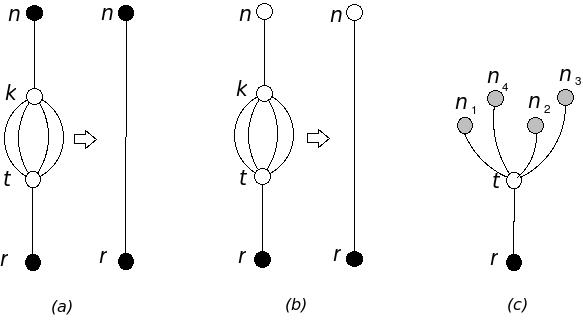
\includegraphics[scale=0.45]{../img/simplification_derefinement.jpg}
    \caption{Simplification through elimination of transition nodes.}
    \label{FIG_SIMPLIFICATION_DEREFINEMENT}
\end{figure}
\vspace{1cm}

In Figure \ref{FIG_SIMPLIFICATION_DEREFINEMENT}, the nodes denoted
by letters $r$, $t$ and $k$ are, respectively, the replacer cell
node, a transition node created during derefinement, and the
transition node which links to the neighbor node $n$ of the original
bunch.

The simplification procedure happens in the following manner:

\begin{enumerate}
 \item If node $r$ has the same refinement level as node $n$, as it
 happens in cases \textit{(a)} and \textit{(b)}, $r$ and $n$ are
 directly linked. Next, nodes $t$ and $k$ are removed from the graph. Notice that the difference between cases \textit{(a)}
 and \textit{(b)} is that in the first $r$ and $n$ have the same type, while in the latter $r$ is a cell node and
 $n$ is a transition node.

 \item If the quadruple connectors of $t$ point to different cells, then no simplification should be done,
 as in case \textit{(c)}, since this means that $n$ and the nodes $n_i$, $1 \leqslant i \leqslant 4$, have different refinement levels
 or are of different types.
\end{enumerate}

Algorithm \ref{SIMPLIFICATION_DEREFINEMENT} executes the simplifying
steps described above. In the third case, each node
$n_{i}$ must point to the transition node $t$. Notice that it is not
necessary to point $t$ to each node $n_{i}$, since this was already
done in Step 4.

The code from Line 13 through 15 does the simplification for case
\textit{(a)}. The pointer of $n$ (\textit{neighborCN}) which points
to $k$ (\textit{auxiliarTN}) must be modified to point to $r$
(\textit{replacerCell}). This pointer is that whose direction is
opposite to the direction of transition node $t$
(\textit{transitionNode}). The elimination of nodes $t$ and $k$
occurs in Lines 32 and 33, respectively.

The simplification of the second case is executed by the code in Lines
16 through 27. As in case \textit{(a)}, the pointer of $n$ (now
designated \textit{neighborTN}) that points to $k$ must be altered
to point to $r$. Since $n$ is a transition node and one cannot know
a priori which of its five pointers points to $k$, an inspection
must be obligatorily done on all pointers of $n$ to find out which
one points to $k$; once this is found, it is modified to point to
$r$. After the linking, nodes $t$ and $k$ are removed from the
graph.

In the third case, each node $n_i$ (designated by the vector
\textit{quadCon}) must point to the transition node $t$. These nodes
may be each either a cell node or a transition node. If it is a
transition node, its single connector is pointed to $t$; if it is a
cell node, the directional pointer whose direction is opposite to
the direction of $t$ is the one which is pointed to $t$. The
distinction between these two cases occurs in Lines 40 through 43.

\alglanguage{pseudocode}
\begin{algorithm}[!ht]
    \caption{Simplification - Derefinement}
    \small{
    \begin{algorithmic}[1]
    \Procedure{simplifyDeref}{transitionNode}
        \State $CellNode\hspace{2mm} replacerCell \gets transitionNode.singleConnector$
        \State $CellNode\hspace{2mm} neighborCN \gets null$
        \State $TransitionNode\hspace{2mm} neighborTN \gets null$
        \State $TransitionNode\hspace{2mm} auxiliarTN \gets null$
        \State $Cell\hspace{2mm} quadCon[4] \gets null$
        \State $char\hspace{2mm} direction \gets transitionNode.direction$

        \State
        \If{all transitionNode's quadruple connectors point to the same cell}
            \State $auxiliarTN \gets transitionNode.quadrupleConnector1$
            \State $replacerCell.getNeighborCell(direction) \gets auxiliarTN.singleConnector$
            \State $neighborType \gets auxiliarTN.singleConnector.type$
            \If{the neighbor cell is a cell node}
                \State $neighborCN \gets auxiliarTN.singleConnector$
                \State $neighborCN.oppositeDirection(direction) \gets replacerCell$
            \Else
                \State $neighborTN \gets auxiliarTN.singleConnector$
                \If{$neighborTN.singleConnector == auxiliarTN$}
                    \State $neighborTN.singleConnector \gets replacerCell$
                \ElsIf{$neighborTN.quadrupleConnector1 == auxiliarTN$}
                    \State $neighborTN.quadrupleConnector1 \gets replacerCell$
                \ElsIf{$neighborTN.quadrupleConnector2  == auxiliarTN$}
                    \State $neighborTN.quadrupleConnector2 \gets replacerCell$
                \ElsIf{$neighborTN.quadrupleConnector3 == auxiliarTN$}
                    \State $neighborTN.quadrupleConnector3 \gets replacerCell$
                \ElsIf{$neighborTN.quadrupleConnector4 == auxiliarTN$}
                    \State $neighborTN.quadrupleConnector4 \gets replacerCell$
                \Else
                    \State $print('Error')$
                \EndIf
            \EndIf
            \State \textbf{delete} $transitionNode$
            \State \textbf{delete} $auxiliarTN$
        \Else \Comment{In this case the neighbor cells are only linked, not simplified ($3^{\textrm rd}$ case)}
            \State $quadCon[0] \gets transitionNode.quadrupleConnector1$
            \State $quadCon[1] \gets transitionNode.quadrupleConnector2$
            \State $quadCon[2] \gets transitionNode.quadrupleConnector3$
            \State $quadCon[3] \gets transitionNode.quadrupleConnector4$
            \For{$i \gets 0$ \textbf{to} $3$}
                \If{$quadCon[i]$ is a transition node}
                    \State $neighborTN \gets quadCon[i]$
                    \State $neighborTN.singleConnector \gets transitionNode$
                \Else \Comment{the neighbor cell is a cell node}
                    \State $neighborCN \gets quadCon[i]$
                    \State $neighborCN.oppositeDirection(direction) \gets transitionNode$
                \EndIf
            \EndFor
        \EndIf
    \EndProcedure
    \end{algorithmic}
    }
    \label{SIMPLIFICATION_DEREFINEMENT}
\end{algorithm}

    \section{The modified Hilbert curve} \label{SEC_HILBERT_CURVE}

The three-dimensional modified Hilbert curve is a space-filling
curve which is used in ALG for its ability to provide an easy,
efficient and predictable way of ordering the cells of the mesh
independently of its irregularity and at the same time for having
the property of making it possible to divide the mesh in relatively
independent sub-meshes (see Figure \ref{FIG_IRREGULAR_CURVE}). Its insensitivity to the irregularity of the
mesh is mainly due to the fact that local changes in the mesh
require only local changes in the curve. This fact also accounts for
its ability to isolate different regions of the mesh. The
subdivision of the mesh into independent regions through the Hilbert
curve allows the potential use of parallel computing, since
different processes can work simultaneously on different cell
groupings.

\begin{figure}[H]
\centering
    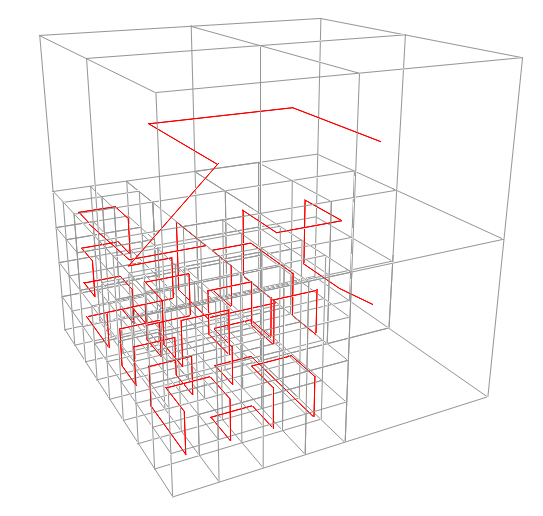
\includegraphics[scale=0.4]{../img/irregularCurve.jpg}
    \caption{Modified Hilbert curve on an irregular mesh.}
    \label{FIG_IRREGULAR_CURVE}
\end{figure}

\subsection{Implementation} \label{SUBSEC_HILBERT_CURVE_IMPLEMENTATION}

The modified Hilbert curve is implemented as a double chain list:
every cell in the mesh, besides having six directional pointers,
possesses also a pointer for the next cell and a pointer for the
previous cell. Thus any cell in the mesh can be reached by
traversing the list until it is located.

\subsubsection{The basic shapes and the Hilbert shape number}
The curve is built recursively by combining $12$ different ways of
ordering the eight cells of a bunch (see Figure
\ref{FIG_BASIC_SHAPES}). Each of these orderings is called a
\textit{basic shape} of the Hilbert curve and constitute the base
cases for the recursion. Initially, one of the basic shapes is
chosen for the ordering of the initial mesh. When one of the cells
of this initial mesh is refined, the new bunch is also ordered
according to one of the $12$ basic shapes. After the ordering, the
segment of curve in the new bunch is connected to the main curve
forming a unique continuous curve.

\begin{figure}[H]
\centering
    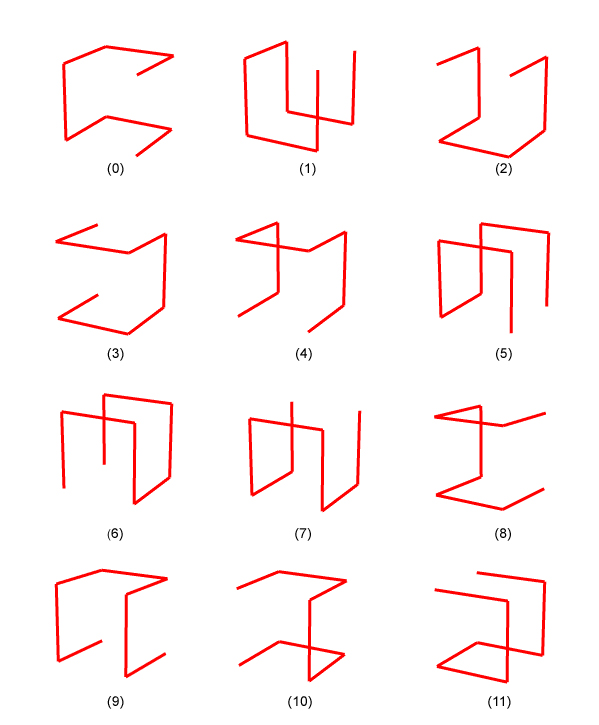
\includegraphics[scale=0.4]{../img/basicShapes.jpg}
    \caption{Basic shapes of the Hilbert curve.}
    \label{FIG_BASIC_SHAPES}
\end{figure}

Each cell in the initial graph stores the number of the basic shape
that will be used in the ordering of the cells in the new bunch in
case it is refined, which is called the \textit{Hilbert shape
number}. When a refinement occurs, the newly created bunch is always
ordered according to the basic shape informed by the refined cell.
Each of the new cells of this bunch also stores the number of the
basic shape which will be used in case the cell itself is also
refined. This way, the modified Hilbert curve is recursively defined
from the $12$ basic shapes. This process does not require the mesh
to be uniformly refined, differently from the traditional Hilbert
curve which works only on regular meshes. The modified Hilbert curve
has the advantage of supporting local changes in the mesh, when only
one cell is refined or only one bunch is derefined.

As an example of this procedure, consider the refinement of cell
number zero in Figure \ref{FIG_INITIAL_HILBERT_CURVE} (a). Upon
refinement, it will be replaced by a bunch that will be ordered
according to the Hilbert shape number stored in the original cell.
For cell zero, this was set to be number 1. After the ordering of
the bunch's cells using the basic shape 1, the main curve and the
segment of curve in the new bunch are connected, resulting in the
curve of Figure \ref{FIG_INITIAL_HILBERT_CURVE} (b).

%HILBERT INICIAL
\begin{figure}[H]
    \centering
    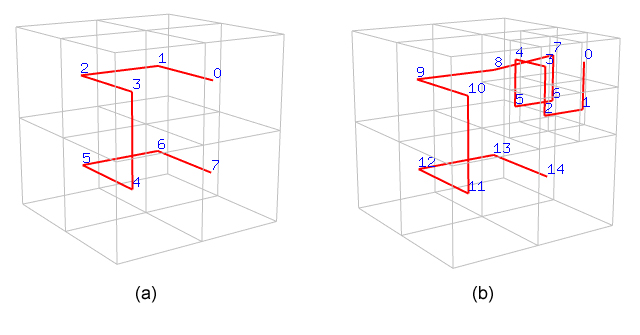
\includegraphics[scale=0.38,angle=0]{../img/initialHilbertCurve.jpg}
    \caption{Example of reordering of mesh cells using the modified Hilbert curve after the refinement of one cell.}
    \label{FIG_INITIAL_HILBERT_CURVE}
\end{figure}

In this work, the convention was made that the cells in the initial
mesh will be always ordered using the basic shape number zero of
Figure \ref{FIG_BASIC_SHAPES}. Afterwards, the way a basic shape
number is assigned to a cell in the mesh depends on the position of
the cell in its bunch and the number of the basic shape that was
used in ordering the bunch.

Table \ref{TAB_ASSIGNEMENTS_OF_BASIC_SHAPES} shows how to define the
Hilbert shape number for each cell in a bunch, given the number of
the basic shape used to order the cells in the bunch to which the
cell belongs and the position of the cell within the bunch. For
instance, if the front southwest (F-SW) cell of a bunch ordered
using basic shape $7$ is refined, then the cells in the bunch that
replaces this cell will be ordered using basic shape $11$;
correspondingly, these new cells will have their Hilbert shape
number set also to $11$.

\begin{acmtable}{320pt}[!ht]
    \begin{center}
        \begin{tabular}{|c|c|c|c|c|c|c|c|c|}
            \hline
                & \textbf{F-NE} & \textbf{F-SE} &\textbf{F-SW}& \textbf{F-NW} & \textbf{B-NE}
                & \textbf{B-SE} & \textbf{B-SW} & \textbf{B-NW} \\
            \hline
            \textbf{0} & 1 & 5 & 3 & 2 & 2 & 4 & 4 & 2 \\
            \hline
            \textbf{1} & 0 & 2 & 2 & 6 & 6 & 7 & 7 & 8 \\
            \hline
            \textbf{2} & 1 & 9 & 10 & 11 & 0 & 0 & 10 & 10 \\
            \hline
            \textbf{3} & 7 & 9 & 9 & 7 & 0 & 0 & 6 & 11 \\
            \hline
            \textbf{4} & 7 & 5 & 6 & 7 & 0 & 0 & 10 & 10 \\
            \hline
            \textbf{5} & 4 & 0 & 11 & 4 & 9 & 8 & 11 & 9 \\
            \hline
            \textbf{6} & 4 & 1 & 10 & 4 & 9 & 1 & 3 & 9 \\
            \hline
            \textbf{7} & 4 & 1 & 11 & 4 & 3 & 11 & 1 & 8 \\
            \hline
            \textbf{8} & 7 & 9 & 9 & 7 & 1 & 5 & 10 & 10 \\
            \hline
            \textbf{9} & 8 & 8 & 3 & 3 & 2 & 5 & 6 & 2 \\
            \hline\
            \textbf{10} & 8 & 8 & 6 & 11 & 2 & 4 & 4 & 2 \\
            \hline
            \textbf{11} & 10 & 10 & 5 & 2 & 3 & 3 & 5 & 7 \\
            \hline
        \end{tabular}
    \end{center}
    \caption{Hilbert shape number assignment to mesh cells.
     Leftmost column refers to basic shape number previously used in ordering the bunch to which the cell belongs.}
    \label{TAB_ASSIGNEMENTS_OF_BASIC_SHAPES}
\end{acmtable}

The Hilbert shape number of each of the cells in the initial mesh is
configured according to the first row in the table, corresponding to
a Hilbert shape number equal to $0$ for the bunch. Thus, the front
northeast (F-NE) cell stores $1$ in its Hilbert shape number, the
front southeast (F-SE) stores $5$, the front southwest stores $3$
and so on.

\subsubsection{Ordering of cells within a bunch}

In this paragraph, it will be shown how the cells of a bunch are
ordered according to each basic shape. This ordering amounts to
determine for each cell of the bunch which cell its \textit{next}
and \textit{previous} pointers will point to. Table
\ref{TAB_DEFINITION_OF_BASIC_SHAPES} describes the ordering chosen
for each basic shape number.

Let $(i, j)$ denote the cell corresponding to the $i$-th row and
$j$-th column in Table \ref{TAB_DEFINITION_OF_BASIC_SHAPES},
$i=0,\ldots , 11$ and $j=1,\ldots , 8$. The ordering of the bunch's
cells according to basic shape $i$ is done by making the
\textit{next} pointer of cell $(i,j)$ point to cell $(i, j+1)$ for
$j=1,\ldots , 7$ and \textit{previous} pointer of cell $(i,j)$ point
to cell $(i, j-1)$ for $j=2,\ldots , 8$. Pointers \textit{previous}
of cell $(i,1)$ and \textit{next} of cell $(i,8)$ are treated
separately since they are responsible for connecting the curve
segment in the bunch to the main curve in the graph making a
continuous curve. Pointer \textit{previous} of cell $(i,1)$ must
point to the cell referenced by pointer \textit{previous} of the
cell which originated the bunch, while pointer \textit{next} of cell
$(i,8)$ must point to the cell referenced by pointer \textit{next}
of the cell which originated the bunch.
\begin{acmtable}{310pt}[!ht]
    \begin{center}
        \begin{tabular}{|c|c|c|c|c|c|c|c|c|}
            \hline
                & \boldmath$1^{\rm st}$ & \boldmath$2^{\rm nd}$ & \boldmath$3^{\rm rd}$ & \boldmath$4^{\rm th}$
                & \boldmath$5^{\rm th}$ & \boldmath$6^{\rm th}$ & \boldmath$7^{\rm th}$ & \boldmath$8^{\rm th}$ \\
            \hline
            \textbf{0} & F-NE & B-NE & B-NW & F-NW & F-SW & B-SW & B-SE & F-SE \\
            \hline
            \textbf{1} & F-NE & F-SE & F-SW & F-NW & B-NW & B-SW & B-SE & B-NE \\
            \hline
            \textbf{2} & F-NE & B-NE & B-SE & F-SE & F-SW & B-SW & B-NW & F-NW \\
            \hline
            \textbf{3} & B-NW & F-NW & F-NE & B-NE & B-SE & F-SE & F-SW & B-SW \\
            \hline
            \textbf{4} & F-SW & B-SW & B-NW & F-NW & F-NE & B-NE & B-SE & F-SE \\
            \hline
            \textbf{5} & B-SE & B-NE & B-NW & B-SW & F-SW & F-NW & B-NE & B-SE \\
            \hline
            \textbf{6} & F-SW & F-NW & F-NE & F-SE & B-SE & B-NE & B-NW & B-SW \\
            \hline
            \textbf{7} & B-NW & B-SW & F-SW & F-NW & F-NE & F-SE & B-SE & B-NE \\
            \hline
            \textbf{8} & B-SE & F-SE & F-SW & B-SW & B-NW & F-NW & F-NE & B-NE \\
            \hline
            \textbf{9} & B-SE & F-SE & F-NE & B-NE & B-NW & F-NW & F-SW & B-SW \\
            \hline
            \textbf{10} & F-SW & B-SW & B-SE & F-SE & F-NE & B-NE & B-NW & F-NW \\
            \hline
            \textbf{11} & B-NW & B-NE & B-SE & B-SW & F-SW & F-SE & F-NE & F-NW \\
            \hline
        \end{tabular}
    \end{center}
    \caption{Ordering of cells within a bunch according to the number of basic shape used.}
    \label{TAB_DEFINITION_OF_BASIC_SHAPES}
\end{acmtable}

\subsection{Hilbert curve in refinement} \label{SUBSEC_HILBERT_CURVE_REFINEMENT}
As seen in Section \ref{SEC_REFINEMENT}, the ordering of the cells
of a new bunch occurs in the refinement procedure (Step 6). After
the creation and linking of the cells of the bunch, the attribute
\textit{hilbertShapeNumber} and pointers \textit{next} and
\textit{previous} are configured for each cell. This is done by
Algorithm \ref{SORTING_REFINEMENT}, where variable \textit{cellNode}
contains a reference for the cell which is being refined.

\alglanguage{pseudocode}
\begin{algorithm}[!ht]
    \caption{Ordering of the cells of a bunch by the modified Hilbert Curve}
    \small{
    \begin{algorithmic}[1]
        \State $i \gets cellNode.hilbertShapeNumber$
        \For{\textbf{each} bunch's cell node}
            \State set current cell's $hilbertShapeNumber$ according to row $i$ of Table
            \ref{TAB_ASSIGNEMENTS_OF_BASIC_SHAPES}
            \State set current cell's $next$ pointer according to row $i$ of Table \ref{TAB_DEFINITION_OF_BASIC_SHAPES}
            \State set current cell's $previous$ pointer according to row $i$ of Table \ref{TAB_DEFINITION_OF_BASIC_SHAPES}
        \EndFor
    \end{algorithmic}
    }
\label{SORTING_REFINEMENT}
\end{algorithm}


\subsection{Hilbert curve in derefinement} \label{SUBSEC_HILBERT_CURVE_DEREFINEMENT}
When a bunch of cells is derefined, the cell which replaces the
bunch must restore the attribute \textit{hilbertShapeNumber} that
the cell which originated the bunch had, so that if this cell is
refined in some later iteration of the algorithm, the cells of the
refined bunch will be ordered in the same way. This way, the mesh
can be repeatedly refined and derefined, always having the cells
ordered in the same way for a given mesh configuration. However,
since the mesh cells do not store this information, it is necessary
to create a mechanism to find the value of the Hilbert shape number
of the originating cell from a combination of the Hilbert shape
numbers of the cells which constitute the bunch. Function
\textit{getFatherHilbertShape()} in Algorithm
\ref{FATHER_HILBERT_SHAPE_PROCEDURE} performs this task using Table
\ref{TAB_ASSIGNEMENTS_OF_BASIC_SHAPES} which gives the sum of Hilbert
shape numbers for the cells in a bunch according to the basic shape
used when ordering them.

One notices in Table \ref{TAB_ASSIGNEMENTS_OF_BASIC_SHAPES} that
there are no identical rows. Thus, the sequence of the Hilbert shape
numbers of the bunch cells could be used as a way to identify the
basic shape utilized in ordering the bunch's cells. On the other
hand, one also notices that the sum of the Hilbert shape numbers of
the bunch's cells are also different in every row, with the
exception of rows 4, 10 and 11, whose sum equals 45 (see Table
\ref{TAB_IDENTIFICATION_OF_HILBERT_SHAPE_FATHER}). Therefore,
instead of using a sequence of 8 numbers, the single number provided
by this sum is used to identify most of the basic shapes; in the
three cases where the sum is 45, one needs only to verify the
Hilbert shape number of the second cell of the bunch (with respect
to the ordering given by Table
\ref{TAB_DEFINITION_OF_BASIC_SHAPES}), since it is different in any
of the basic shapes 4, 10 and 11.

\begin{acmtable}{310pt}[!ht]
    \begin{center}
        \begin{tabular}{|l|c|c|c|c|c|c|c|c|c|c|c|c|}
            \hline
               \textbf{Basic shape} & 0 & 1 & 2 & 3 & 4 & 5 & 6 & 7 & 8 & 9 & 10 & 11 \\
            \hline
               \textbf{Sum} & 24 & 38 & 50 & 49 & 45 & 56 & 41 & 43 & 58 & 37 & 45 & 45 \\
            \hline
        \end{tabular}
    \end{center}
    \caption{Sum of Hilbert shape numbers for the cells in a bunch according to each basic shape.}
    \label{TAB_IDENTIFICATION_OF_HILBERT_SHAPE_FATHER}
\end{acmtable}

\alglanguage{pseudocode}
\begin{algorithm}[!ht]
    \caption{Returns the Hilbert's basic shape of a given bunch upon receiving the bunch's first cell as a parameter}
    \small{
    \begin{algorithmic}[1]
        \Procedure{getFatherHilbertShape}{firstBunchCell}
            \State $sum \gets 0$
            \State $hilbertShape \gets -1$
            \State $auxiliarCell \gets firstBunchCell$
            \State
            \For{i $\gets$ 1 \textbf{to} 8}
                \State $sum \gets sum + auxiliarCell \cdot hilbertShapeNumber$
                \State $auxiliarCell \gets auxiliarCell \cdot next$
            \EndFor
            \State
            \If{$sum == 24$}
                \State $hilbertShape \gets 0$
            \ElsIf{$sum == 38$}
                \State $hilbertShape \gets 1$
            \ElsIf{$sum == 50$}
                \State $hilbertShape \gets 2$
            \ElsIf{$sum == 49$}
                \State $hilbertShape \gets 3$
            \ElsIf{$sum == 45$}
                \If{$firstBunchCell \cdot next \cdot hilbertShapeNumber == 10$}
                    \State $hilbertShape \gets 4$
                \ElsIf{$firstBunchCell \cdot next \cdot hilbertShapeNumber == 4$}
                    \State $hilbertShape \gets 10$
                \Else
                    \State $hilbertShape \gets 11$
                \EndIf
            \ElsIf{$sum == 56$}
                \State $hilbertShape \gets 5$
            \ElsIf{$sum == 41$}
                \State $hilbertShape \gets 6$
            \ElsIf{$sum == 43$}
                \State $hilbertShape \gets 7$
            \ElsIf{$sum == 58$}
                \State $hilbertShape \gets 8$
            \ElsIf{$sum == 37$}
                \State $hilbertShape \gets 9$
            \Else
                \State $print('Error')$
            \EndIf
            \State
            \Return $hilbertShape$
        \EndProcedure
    \end{algorithmic} \label{FATHER_HILBERT_SHAPE_PROCEDURE}
    }
\end{algorithm}

    \section{Application on cardiac electrophysiology simulation}

Simulations of cardiac electrophysiology have become a valuable tool for the
study and comprehension of the heart's bioelectric activity under normal and
pathological conditions. These simulations are usually based on the bidomain
model~\cite{Sundnes2006Book}, which is a system of two partial differential
equations (PDEs) coupled to a set of nonlinear ordinary differential equations
(ODEs) describing the behavior of the membrane of cardiac cells. In spite of
being currently the most complete description of the electrical activity of the
heart, the numerical solution of the bidomain equations is a computational
challenging task~\cite{Weber2004}. Usually the bidomain equations are reduced to
the simpler monodomain model by considering that: the extracellular potential is
constant; or tissue conductivity is isotropic; or the intracellular and
extracellular conductivities have equal anisotropy
ratios~\cite{Sundnes2006Book}.

\subsection{Monodomain Model}

In cardiac tissue, the excitation wave spreads through the tissue because
the cardiac cells are electrically coupled via special proteins called
gap junctions. This phenomenon is mathematically described by a
reaction--diffusion equation referred to as the monodomain equation, given by
\begin{align}
   \beta C_m \DP{V_m}{t} + \beta I_{ion}(V_m,\bs{\eta}) &=
   \nabla \cdot (\bs{\sigma_m} \nabla V_m) + I_{stim}\\
\DP{\bs{\eta}}{t} &= \bs{f}(V_m, \bs{\eta})
   \label{eq:Monodomain}
\end{align}
where $\beta$ is the surface-to-volume ratio of the cardiac cells,
$C_m$ is the membrane capacitance, $V_m$ is the transmembrane voltage,
$I_{ion}$ is the density of the total ionic current which is a function of
$V_m$ and a vector of state variables $\bs{\eta}$, $I_{stim}$ is a stimulus
current and $\bs{\sigma_m}$ is the monodomain conductivity tensor. The tissue
is assumed to be isolated along its boundaries, i.e. no--flux boundary
conditions are imposed on $V_m$ along all myocardial surfaces.

In this work the classical Luo--Rudy I (LRI) model~\cite{Luo1991} that describes the
electrical activity in a general mammalian ventricular cell was considered to
simulate the kinetics of $I_{ion}$ in Eq.~\eqref{eq:Monodomain}. In this
mammalian ventricular model, $I_{ion}$ is defined as the following sum of
currents:
\begin{equation}
   I_{ion} = I_{Na} + I_{si} + I_{K} + I_{K1} + I_{Kp} + I_{b}
   \label{eq:LRDI}
\end{equation}
where $I_{Na}$ is the fast sodium current, $I_{si}$ is the slow inward current,
$I_{K}$ is the time-dependent potassium current, $I_{K1}$ is the
time-independent potassium current, $I_{Kp}$ is the plateau potassium current
and $I_{b}$ is time-independent background current. The LRI model is based on a
set of 8 ODEs describing ionic currents and intracellular calcium concentration.
For a full specification of the model and its ionic currents see~\cite{Luo1991}.

\subsection{Finite Volume model applied to monodomain}

In this section we will make a brief description of the Finite Volume Method (FVM) applied to the
monodomain equations. Details about the FVM applied to monodomain can be found
in~\cite{harrild1997finite} and ~\cite{coudiere20092d}.

The reaction and diffusion part of the monodomain equations can be split by
employing the Godunov operator splitting~\cite{Sundnes2006Book}. Each time step involves the solution of two different problems: a nonlinear system of ODEs
\begin{align}
  \DP{V_m}{t} &= \frac{1}{C_m} \left[ - I_{ion} (V_m,\eta_i) + I_{stim} \right]
  \label{eq:Step1a} \\
  \DP{\eta_i}{t} &= f(V_m, \eta_i) \label{eq:Step1b}
\end{align}
 and a parabolic linear PDE
\begin{align}
  \DP{V_m}{t} &= \frac{1}{\beta C_m}
  \displaystyle\left[ \nabla \cdot (\bs{\sigma} \nabla V_m) \right]
  \label{eq:Step2}
 \end{align}

Depending on the numerical method, the spatial discretization
of the parabolic PDE results in a linear system of equations
that have to be solved at each time step.

\subsubsection{Time discretization}

The time derivative present in Equation~\eqref{eq:Step2}, which operates on $V$
is approximated by an implicit first--order Euler scheme:
\begin{equation}
\frac{\partial V}{\partial t} = \frac{V^{n+1}-V^{n}}{\Delta t},
\label{eq:tempo}
\end{equation}
where $V^{n}$ represents the transmembrane potential at time
$t_{n} $ and $\Delta t$ the increment at every step.

\subsubsection{Space discretization}

The diffusion term of Equation~\eqref{eq:Step2} needs to be spatially
discretized. To do this we will consider the following relations:
\begin{equation}
  J = -\sigma \nabla V
  \label{eq:ji}
\end{equation}
where $J$ $(\mu A/cm^2)$ represents the density of the intracellular current
flow and
\begin{equation}
  \nabla \cdot J = -I_v.
  \label{eq:iv}
\end{equation}

In this expression, $I_v (\mu A/cm^3)$ is a volumetric current and corresponds
the left side of Equation~\eqref{eq:Step2}.

For simplicity, we will consider a tri-dimensional uniform mesh, consisting  of
cubes (called ``Volume''). Situated in the center of each volume
is a node and $V$ is associated with each node of the mesh.

After defining the geometry of the mesh and the partitioning of the domain
in control volumes, the FMV-specific equations can be presented.
The Equation ~\eqref{eq:iv} can be integrated spatially over a cube
specific, leading to:

\begin{equation}
  \int_{\Omega} \nabla \cdot J da = -\int_{\Omega} I_v \, da.
\end{equation}
applying the divergence theorem, we find that
\begin{equation}
  \int_{\Omega} \nabla \cdot J da = \int_{\partial \Omega} J \cdot \vec{\eta},
\end{equation}
where $\vec{\eta}$ is the vector normal to the edge.

Finally, assuming that $ I_v$ represents an average value in each particular
cube, and substituting in Eq~\eqref{eq:Step2}, we have the following
relationship:
\begin{equation}
    \beta\left (C_m \dfrac{\partial V}{\partial t} \right)\bigg|_{(i,j,k)}
     = \dfrac{-\int_{\partial \Omega} J \cdot \vec{\eta}}{h^3},
     \label{eq:mono2}
\end{equation}
where $h^3 $ is the volume of the control cell and $\vec{\eta}$
represents the vector normal to the surface.

For the three-dimensional problem, formed by a uniform grid of cubes with
face area $h^2$, the calculation of $J$ can be split as the sum of the flows
on the six faces:
\begin{equation}
          \int_{\partial \Omega} J \cdot \vec{\eta} = h^2 \cdot \displaystyle
          \sum_{l=1}^{6}{{Jf}_l}
     \label{eq:flux}
\end{equation}
where,
\begin{eqnarray}
  \sum_{l=1}^{6}{{Jf}_l} &=& J_{x_{i+1/2,j,k}} - J_{x_{i-1/2,j,k}} \nonumber \\
                      &+& J_{y_{i,j+1/2,k}} - J_{y_{i,j-1/2,k}} \\
                      &+& J_{z_{i,j, k+1/2}} - J_{z_{i,j, k-1/2}} \nonumber,
\end{eqnarray}

The tensor $\sigma = \left(\begin{array}{ccc} \sigma_x & 0 & 0 \\ 0 & \sigma_y &
0 \\ 0 & 0 & \sigma_z \end{array} \right)$ must be determined at the interfaces
of the volume. For this, we use the harmonic mean:
\begin{eqnarray}
    \sigma_{x_{i+1/2, j}} = \displaystyle \dfrac{2\sigma_{x_{i,j}}\sigma_{x_{i+1,j}}}{\sigma_{x_{i+1, j}}+\sigma_{x_{i,j}}}
     % \sigma_{x_{i-1/2, j}} = \displaystyle \dfrac{2\sigma_{x_{i,j}}\sigma_{x_{i-1,j}}}{\sigma_{x_{i-1, j}}+\sigma_{x_{i,j}}}.
\end{eqnarray}

A similar reasoning can be used to calculate $\sigma_{x_{i-1/2, j,
k}}$, $\sigma_{y_{i, j+1/2, k}}$, $\sigma_{y_{i, j-1/2}}$, $\sigma_{z_{i, j,
k+1/2}}$ and $\sigma_{z_{i, j, k-1/2}}$.

The flows $J_{x_{m,n,o}}$, $J_{y_{m,n,o}}$ and $J_{y_{m,n,o}}$ are calculated in the
faces ($(m,n,o)$ = $(i+1/2,j,k)$, $(i-1/2,j,k)$, $(i,j+1/2,k)$, $(i,j-1/2,k)$,
$(i,j,k+1/2)$ or $(i,j,k-1/2)$) as follows:

\begin{eqnarray}
    J_{x_{m,n,o}} = \sigma_x(m,n,o) \dfrac{\partial V}{\partial x} \bigg|_{(m,n,o)}\\
    J_{y_{m,n,o}} = \sigma_{y}(m,n,o) \dfrac{\partial V}{\partial y} \bigg|_{(m,n,o)}\\
    J_{z_{m,n,o}} = \sigma_{z}(m,n,o) \dfrac{\partial V}{\partial z} \bigg|_{(m,n,o)}
\end{eqnarray}

\subsubsection{Adaptive non-uniform mesh (ALG)}

In this section we present the application of the FVM using an adaptive non-
uniform mesh, in this case ALG. For this, we will approximate the partial derivatives of $V$ on
the interfaces using the following finite difference scheme, considering uniform
discretizations in space ($\Delta x = \Delta y = \Delta z = h$):
\begin{eqnarray}
    \label{eq:dvdx1}
    \dfrac{\partial V}{\partial x} \bigg|_{(i+1/2,j,k)} = \dfrac{V_{i+1,j,k} - V_{i,j,k}}{h}
\end{eqnarray}
The equations for $y$ and $z$ can be obtained similarly.

Rearranging and replacing the discretizations of the equations~\eqref{eq:tempo}
and~\eqref{eq:flux} in Equation~\eqref{eq:mono2} and decomposing the
operators as described by the equations~\eqref{eq:Step1a}, \eqref{eq:Step1b} and~
\eqref{eq:Step2} we have:
\begin{eqnarray}
C_m \dfrac{V^{*}_{i,j,k} - V^{n}_{i,j,k}}{\Delta t} &=&\dfrac{h^2 \cdot \displaystyle
          \sum_{l=1}^{6}{{Jf^*}_l} }{\beta h^3} \\
C_m \dfrac{V^{n+1}_{i,j,k} - V^{*}_{i,j,k}}{\Delta t} &=& -I_{ion}(V^*_{i,j,k},\bs{\eta}^n) \\
\dfrac{\partial \bs{\eta}^{n+1}}{\partial t} &=& f(\bs{\eta}^n, V^*, t)
\end{eqnarray}
where:
\begin{eqnarray}
%%%%%%J_{i+1/2,j}%%%%%%%%%%
   J^*_{x_{i+1/2,j}} =
   \sigma_{x_{i+1/2,j,k}} \dfrac{V^{*}_{i+1,j,k} - V^{*}_{i,j,k}}{h},
   \label{eq:fluxo1}
\end{eqnarray}
Eq.~\eqref{eq:fluxo1} represents the flow of the cell (i, j, k) by the right
face of the cube to the neighbor cell, $n$ is the current step, $*$ is
an intermediate step and $n+1$ is the next time step. Equations for
$J^*_{x_{i-1/2,j,k}}$, $J^*_{y_{i,j+1/2,k}}$, $J^*_{y_{i,j-1/2,k}}$,
$J^*_{z_{i,j, k+1/2}}$ and $J^*_{z_{i,j, k-1/2}}$ can be obtained similarly.
Developing all equations, we can now define the time advance formula for
the interior points of each volume:
\begin{align}
\label{eq:sis_so}
\nonumber
(\sigma_{x_{i+1/2,j,k}}+\sigma_{x_{i-1/2,j,k}} +\sigma_{y_{i,j+1/2,k}} + \sigma_{y_{i,j-1/2,k}} \sigma_{x_{i,j,k+1/2}}+\sigma_{x_{i,j,k-1/2}} + \alpha) V^*_{i,j,k} + \\ \nonumber
\sigma_{y_{i,j-1/2,k}} V^*_{i,j-1,k} -\\ \nonumber
\sigma_{x_{i+1/2,j,k}} V^*_{i+1,j,k} -\\ \nonumber
\sigma_{z_{i,j,k+1/2}} V^*_{i,j,k+1} -\\ \nonumber
\sigma_{y_{i,j+1/2,k}} V^*_{i,j+1,k} -\\ \nonumber
\sigma_{x_{i-1/2,j,k}} V^*_{i-1,j,k}  =
V^t_{i,j,k}*\alpha,
\end{align}
where $\alpha = (\beta C_m h^2)/\Delta t$.

Algorithm \ref{mono_alg} describes the steps used for the numerical resolution
of monodomain model. As can be seen, we have to reassemble the monodomain
matrix at each time step if a refinement or derefinement operation has been
performed in that step. In this example application, the criteria used for
refinement and derefinement are based on the flux across the interface of
neighboring cells. That is, if the absolute value of the flux is larger than a
predefined refinement threshold ($reft$), the program chooses to refine this
cell, whereas if the absolute value of the flux of all four cells of a bunch is
less than an derefinement threshold ($dreft$), the program chooses to derefine
the bunch. For the monodomain application, the values for the refinement and
derefinement thresholds where empirically found.
\alglanguage{pseudocode}
\begin{algorithm}[!ht]
    \caption{Steps used for the numerical resolution of monodomain model}
    \small{
    \begin{algorithmic}[1]
        \State set cell model initial conditions;
        \State assemble the monodomain matrix (Linear system form PDE);
        \While{$t < final\_t$}
        \State update cell Model state vector;
        \State solve cell model;
       \State solve linear system (PDE) via conjugate gradient method;
        \State refine-derefine
       \State reassemble the monodomain matrix if needed;
       \State $t = t + dt$
        \EndWhile
    \end{algorithmic}
    }
    \label{mono_alg}
\end{algorithm}

Figure~\ref{SIM_ALG3D} shows the simulation results using ALG adaptive mesh. We can
clearly see that the region delimited by the wavefront has a spatial discretization
smaller than the rest of the tissue. The colors represents the distribution of
transmembrane potential V.

\begin{figure}
    \centering
    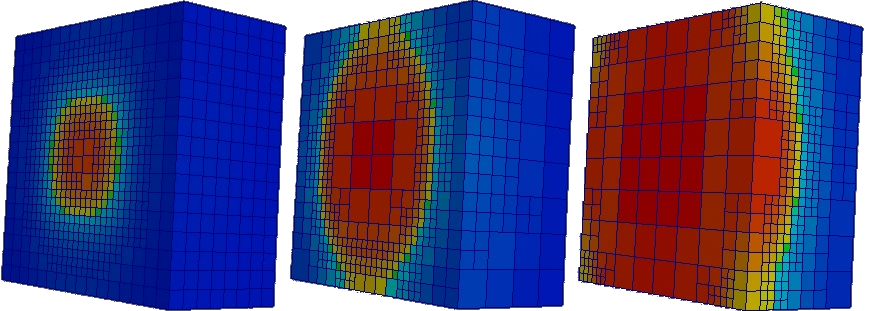
\includegraphics[scale=0.40]{../img/onda3d.png}
    \caption{Simulation using ALG adaptivity scheme. Result of the simulated
electric wave propagation (distribution of transmembrane potential V ) in a ventricular
tissue.}
    \label{SIM_ALG3D}
\end{figure}

    %\begin{thebibliography}{99}

\bibitem[Burgarellio 1998]{Burgarelli1998} BURGARELLI, D. \textit{Modelagem computacional e
simula\c c\~ao num\'erica adaptativa de equa\c c\~oes diferenciais
parciais evolutivas aplicadas a um problema termoac\'ustico}, Ph.D. thesis, PUC-Rio, Rio de Janeiro, Brasil, (1998). (in
Portuguese)

\bibitem[Burgarelli et al. 2006]{Burgarellietal2006}BURGARELLI, D., KISCHINHEVSKY, M. and BIEZUNER, R. J.,
A new adaptive mesh refinement strategy for numerically solving
evolutionary PDE's, \textit{Journal of Computational and Applied
Mathematics} \textbf{196} (2006) 115--131.


\bibitem[Gamezo et al. 2005a]{Gamezoetal2005a}  GAMEZO, V. N.,  KHOKHLOV, A. M. and ORAN, E.S.,
Three-dimensional delayed-detonation model of type Ia supernovae, \textit{The Astrophysical Journal} \textbf{623} (2005) 337-346.


\bibitem[Gamezo et all. 2005b]{Gamezoetal2005b}  GAMEZO, V. N., ORAN , E. S. and   KHOKHLOV, A. M.,
Three-dimensional reactive shock bifurcations, \textit{Proceedings of the Combustion Institute .} \textbf{30} (2005) 1841-1847.


\bibitem[Ji et all. 2008]{Jietal2008}  JI, H., LIEN, F. and   YEE, E.,
A robust and efficient hybrid cut-cell/ghost-cell method with adaptive mesh refinement for moving boundaries on irregular domains, \textit{Comput. methods Appl. Mech. Engrg.} \textbf{198} (2008) 432-448.


\bibitem[Penner et all. 2007]{Penneretal2007}  PENNER, J. E., ANDRONOVA, N.,  OEHMKE,R.C., BROWN,J., STOUT, Q.F., JABLONOWSKI, C., VAN LEER, B., POWELL, K.G. and  HERZOG, M.,
Three Dimensional adaptive mesh refinement on a spherical shell for atmospheric  models with lagrangian coordinates, \textit{Journal of Physics : Conference Series .} \textbf{78} (2007) 1-5.



\bibitem[Tavakoli 2006]{tavakoli2006} TAVAKOLI, R.,
CartGen: Robust, efficient and easy to implement uniform/octree/embedded boundary Cartesin grid generator, \textit{International Journal for Numerical Methods in Fluids} \textbf{57} (2008) 1753--1770.



\end{thebibliography}

    \bibliographystyle{acmtrans}
    \bibliography{bibliography}

\end{document}
